\documentclass[12pt]{article}
\usepackage[utf8]{inputenc}
\usepackage{listings}
\usepackage{xcolor}
\usepackage{graphicx}
\usepackage{amsmath}
\usepackage{hyperref}
\usepackage[
backend=biber,
style=alphabetic,
sorting=ynt
]{biblatex}

\definecolor{codegreen}{rgb}{0,0.6,0}
\definecolor{codegray}{rgb}{0.5,0.5,0.5}
\definecolor{codepurple}{rgb}{0.58,0,0.82}
\definecolor{backcolour}{rgb}{0.95,0.95,0.92}
\lstdefinestyle{mystyle}{
    backgroundcolor=\color{backcolour},   
    commentstyle=\color{codegreen},
    keywordstyle=\color{magenta},
    numberstyle=\tiny\color{codegray},
    stringstyle=\color{codepurple},
    basicstyle=\ttfamily\footnotesize,
    breakatwhitespace=false,         
    breaklines=true,                 
    captionpos=b,                    
    keepspaces=true,                 
    numbers=left,                    
    numbersep=5pt,                  
    showspaces=false,                
    showstringspaces=false,
    showtabs=false,                  
    tabsize=2
}

\lstset{style=mystyle}
\begin{document}
\title{CSDS 391 Programming Assignment 2 Writeup}
\author{Ningjia Huang, Tianxi Zhao}
\date{Due On: December 4, 2020}
\maketitle

\section*{Problem 1: }
\subsection*{(a)}
The plot of 2nd and 3rd classes of the dataset with petal length v.s. petal width is as following:
\begin{center}
    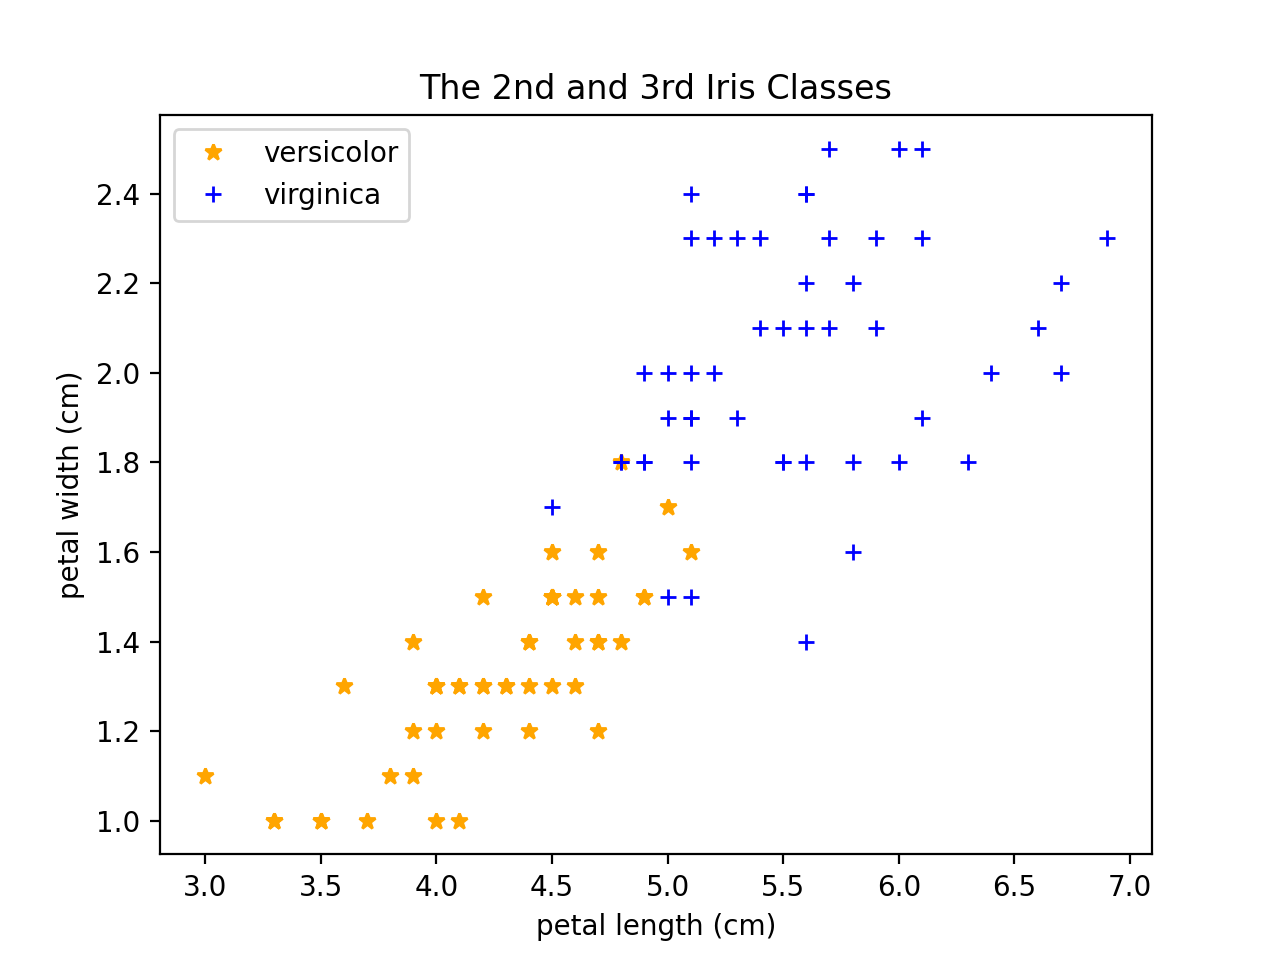
\includegraphics[scale=0.50]{fig/ai1a}
\end{center}
The plot of 2nd and 3rd classes of the dataset with sepal length vs. sepal width:
\begin{center}
    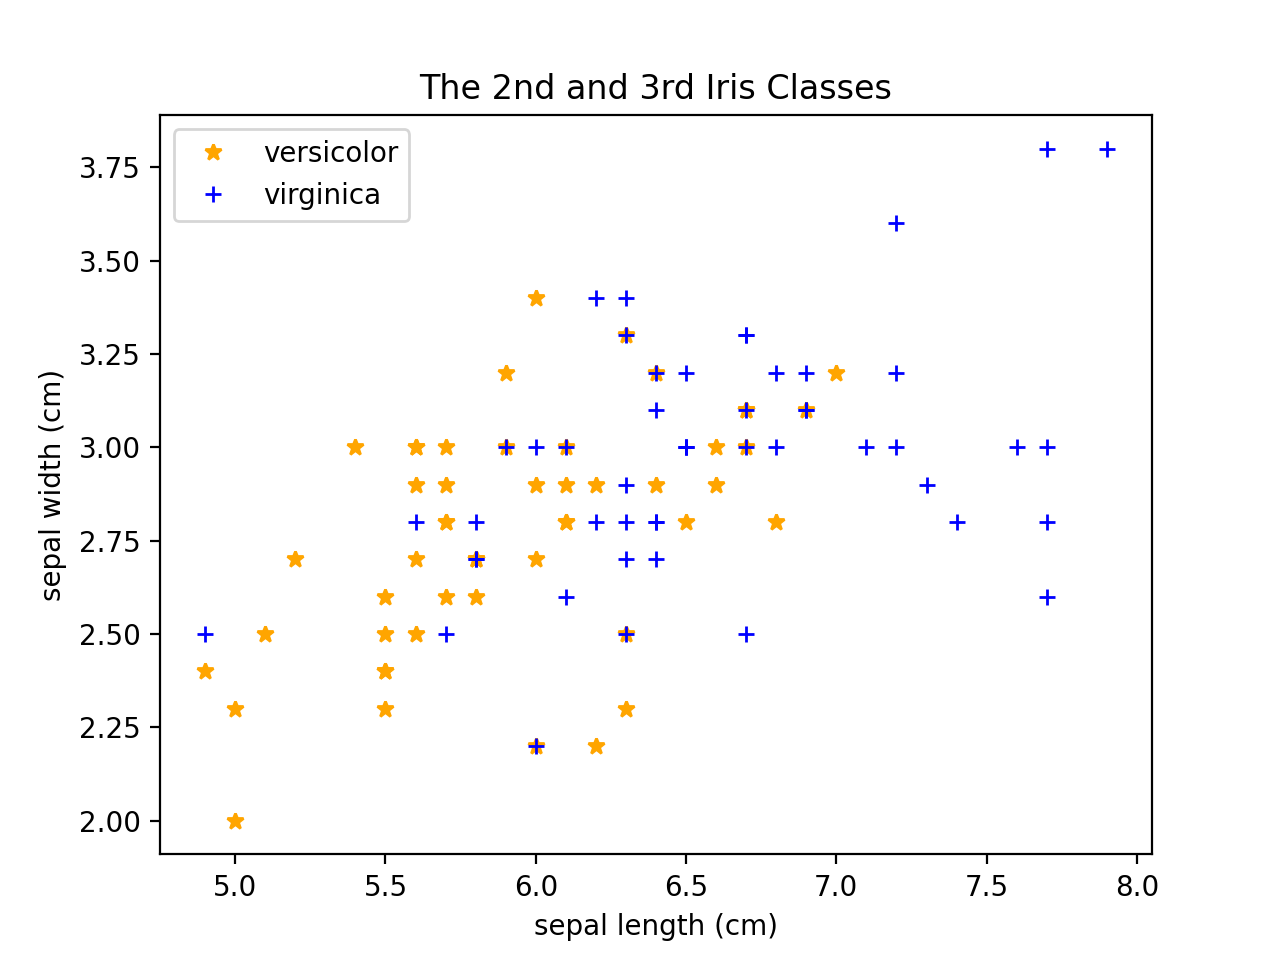
\includegraphics[scale=0.50]{fig/ai1a2}
\end{center}
We can see that petal width vs. petal length can better seperate the 2nd and 3rd classes.

\subsection*{(b)}
We define the output unit: y = $w_1 \cdot$ petal\_length + $w_2 \cdot$ petal\_width + $w_0$
$w_1$ and $w_2$ are weigths, $w_0$ is bias.
The sigmoid function is: 
\begin{center}
    $sigmoid = \dfrac{1}{1 + e^{-y}}$

\end{center}
The following code implements the sigmoid function: 
\begin{center}
    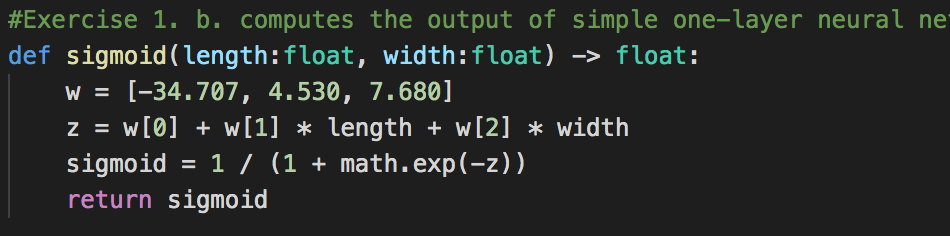
\includegraphics[scale=0.50]{fig/ai1b2}
\end{center}
Implementation of Decision Boundary:
\begin{center}
    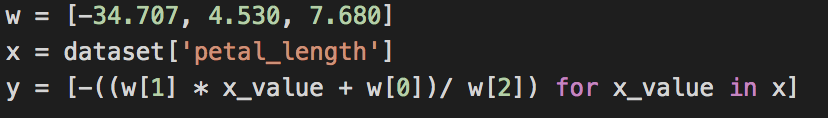
\includegraphics[scale=0.50]{fig/ai1c2}
\end{center}

\subsection*{(c)}
Because the output unit is y = $w_1 \cdot$ petal\_length + $w_2 \cdot$ petal\_width + $w_0$ and the decision boundary is when y = 0, 
we use $x_1$ to represent petal length and $x_2$ to represent petal width: 
\begin{center}
    0 = $w_1 \cdot x_1 + w_2 \cdot x_2 + w_0$ \\ 
    $x_2 = -\dfrac{w_1 \cdot x_1 + w_0}{w_2}$
\end{center}
Decision Boundary Code:
\begin{center}
    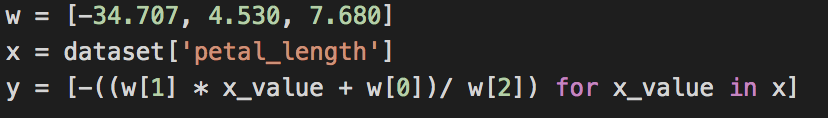
\includegraphics[scale=0.50]{fig/ai1c2.png}
\end{center}
We draw the decision boundary on the graph using python: $plt.plot(x_1, x_2)$
\begin{center}
    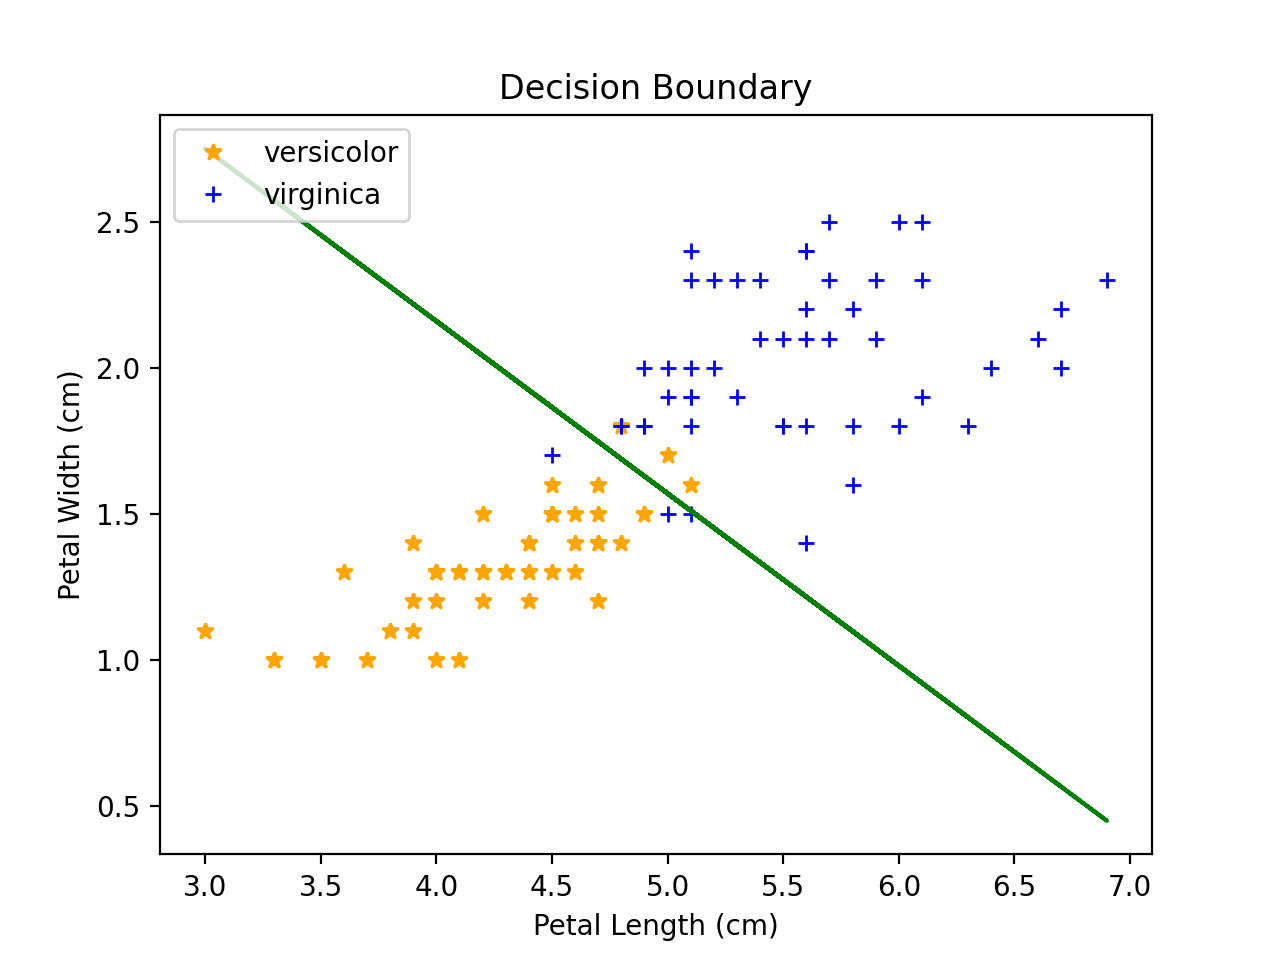
\includegraphics[scale=0.50]{fig/ai1c.png}
\end{center}

\subsection*{(d)}
From the graph generated in (a), we can see that the range of petal length is from about 3.0 to 7.0 cm and the range of petal width is from about 1.0 to 2.5 cm,
so we set the range of petal length from 3.0 to 7.0 cm and the range of petal width from 1.0 to 2.5 cm for the surface that we are going to draw. \\
Then we use the output function we defined in (b) to calculate the output of each pair of petal length and petal width. \\
Code to prepare petal length, petal wieth, and the output:
\begin{center}
    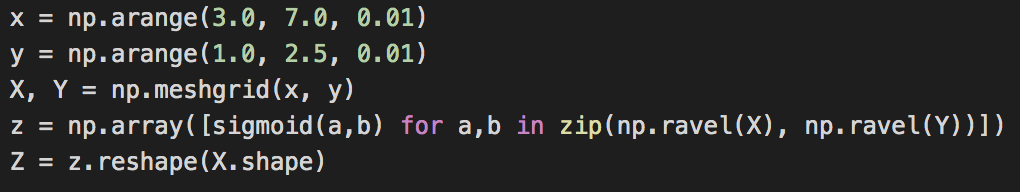
\includegraphics[scale=0.50]{fig/ai1d2.png}
\end{center}
We use the petal length, petal wieth, and the output to draw a 3D neural network:
\begin{center}
    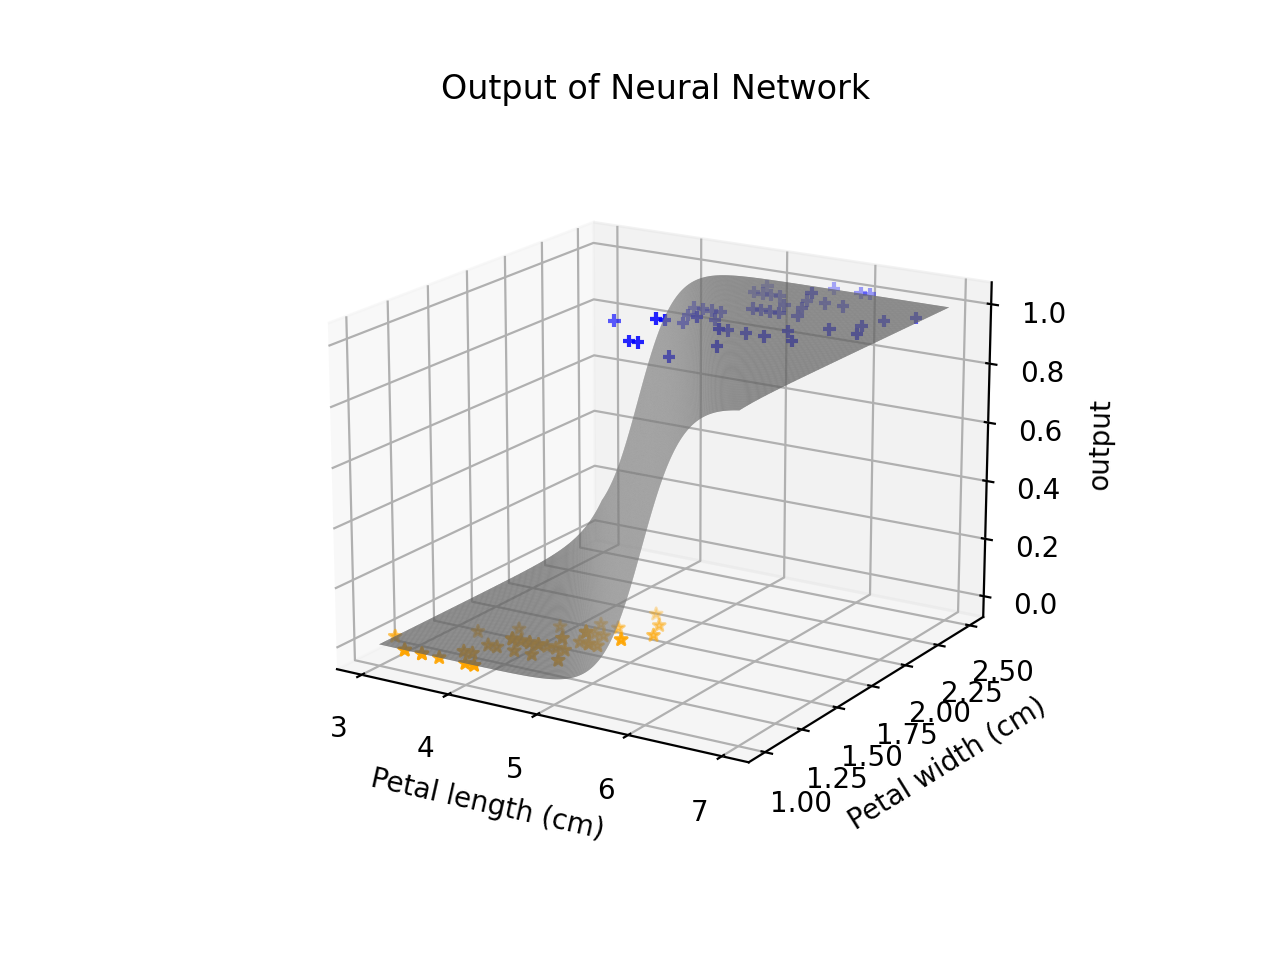
\includegraphics[scale=0.50]{fig/ai1d.png}
\end{center}

\subsection*{(e)}
We selected 8 examples:
\begin{center}
    \begin{tabular}{|l l l|}
        \hline
        petal length (cm) & petal width (cm) & species\\
        \hline
        4.8 & 1.8 & versicolor\\
        5.0 & 1.7 & versicolor\\
        3.5 & 1.0 & versicolor\\
        3.8 & 1.1 & versicolor\\
        5.1 & 1.8 & virginica \\
        5.0 & 1.5 & virginica \\
        4.9 & 1.8 & virginica \\
        5.9 & 2.3 & virginica \\
        \hline
    \end{tabular}
\end{center}

\begin{center}
    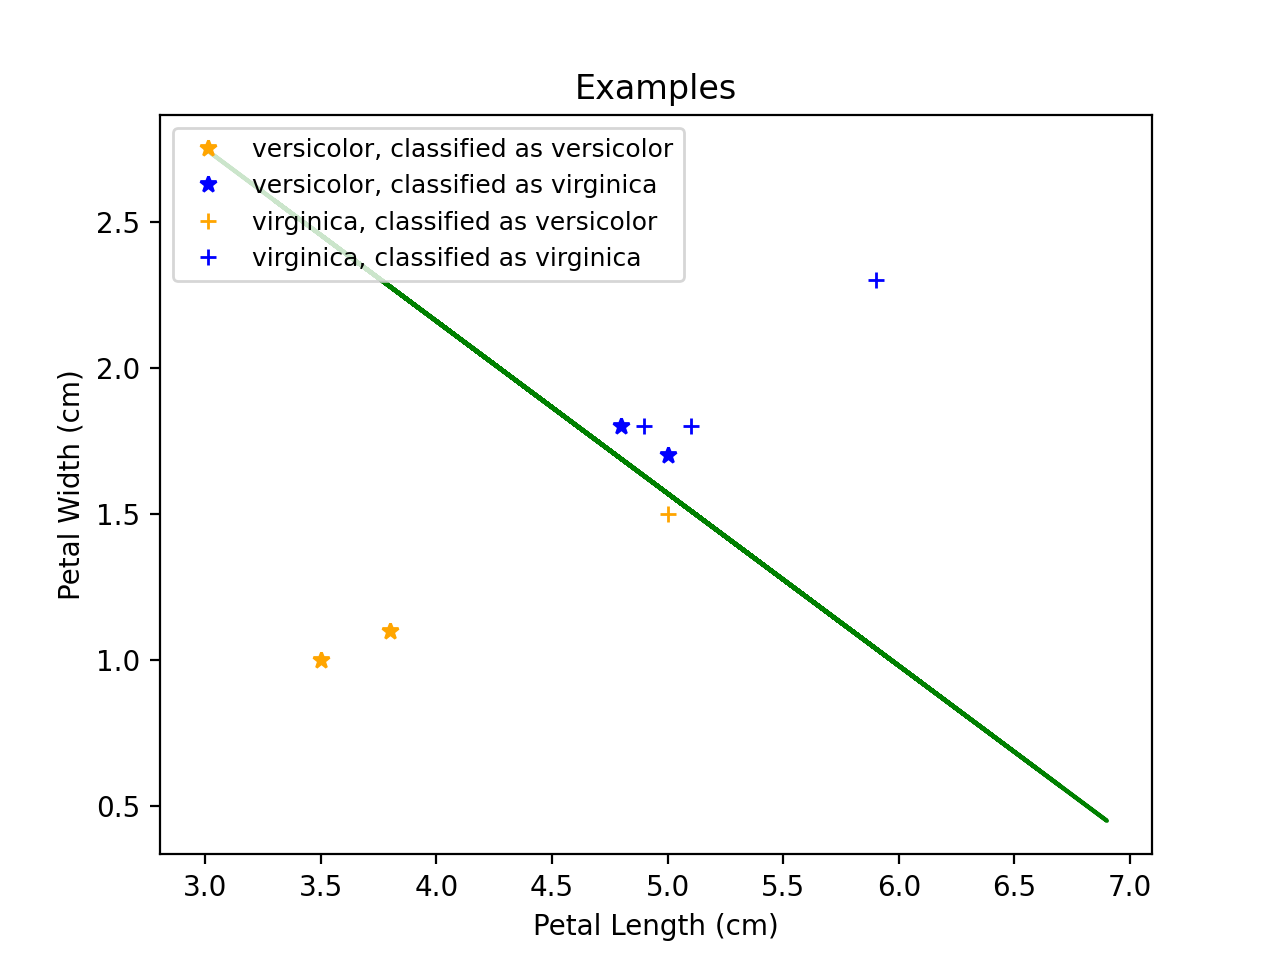
\includegraphics[scale=0.50]{fig/ai1e.png}
\end{center}

\section*{Problem 2: }
\subsection*{(a)}
The mean squared error is calculated using the following equation: 
\begin{center}
    $MSE = \frac{1}{n}\sum_n (Y_i - \hat{Y_i})^2$
\end{center}
, where $Y_i$ is the actual category of the $ith$ item and $\hat{Y_i}$ is the predicted category by using our neural network.\\ \\
The following codes compute the \textbf{mean squared error} for iris data. The parameter "data\_vector" are the attributes we would like to take into account, it should be a dataframe of attributes.
$w_0, w_1, w_2$ define the weights of neural network. The parameter "pattern\_classes" is a dataframe of the category corresponding to the data\_vectors. The \textbf{mean\_square\_error} makes use of 
the logistic non-linearity function in Problem 1.
\begin{lstlisting}[language=Python, caption=Mean Squared Error Calculation]
# data vectors in dataframe, pattern classes in list
def mean_square_error(data_vectors, w0, w1, w2, pattern_classes):
    n = data_vectors.shape[0]
    data_vectors_list = data_vectors.values.tolist()
    pattern_classes_list = pattern_classes.tolist()
    temp_mse = 0
    for i in range(n):
        temp_mse = temp_mse + np.square(pattern_classes_list[i] - one_layer_network(w0, w1, w2, data_vectors_list[i][0], data_vectors_list[i][1]))
    mse = temp_mse/n
    return mse
\end{lstlisting}

\subsection*{(b)}
To plot the linear boundary, we find the x-intercept and y-intercept by using the following code: 
\begin{lstlisting}[language=Python, caption=Plot Mean Squared Error]
plot([0,-w0/w1],[-w0/w2,0])
\end{lstlisting}
\subsubsection*{2.b.1}
The first set of weights we've chosen is $[-3.9, 0.46, 0.95]$. The mean squared error we concluded is 0.13235245817007218. The following figure shows the linear boundary with our chosen set of weights. As we can tell from the graph, the
linear boundary generally seperates the two categories of iris. 
\begin{center}
    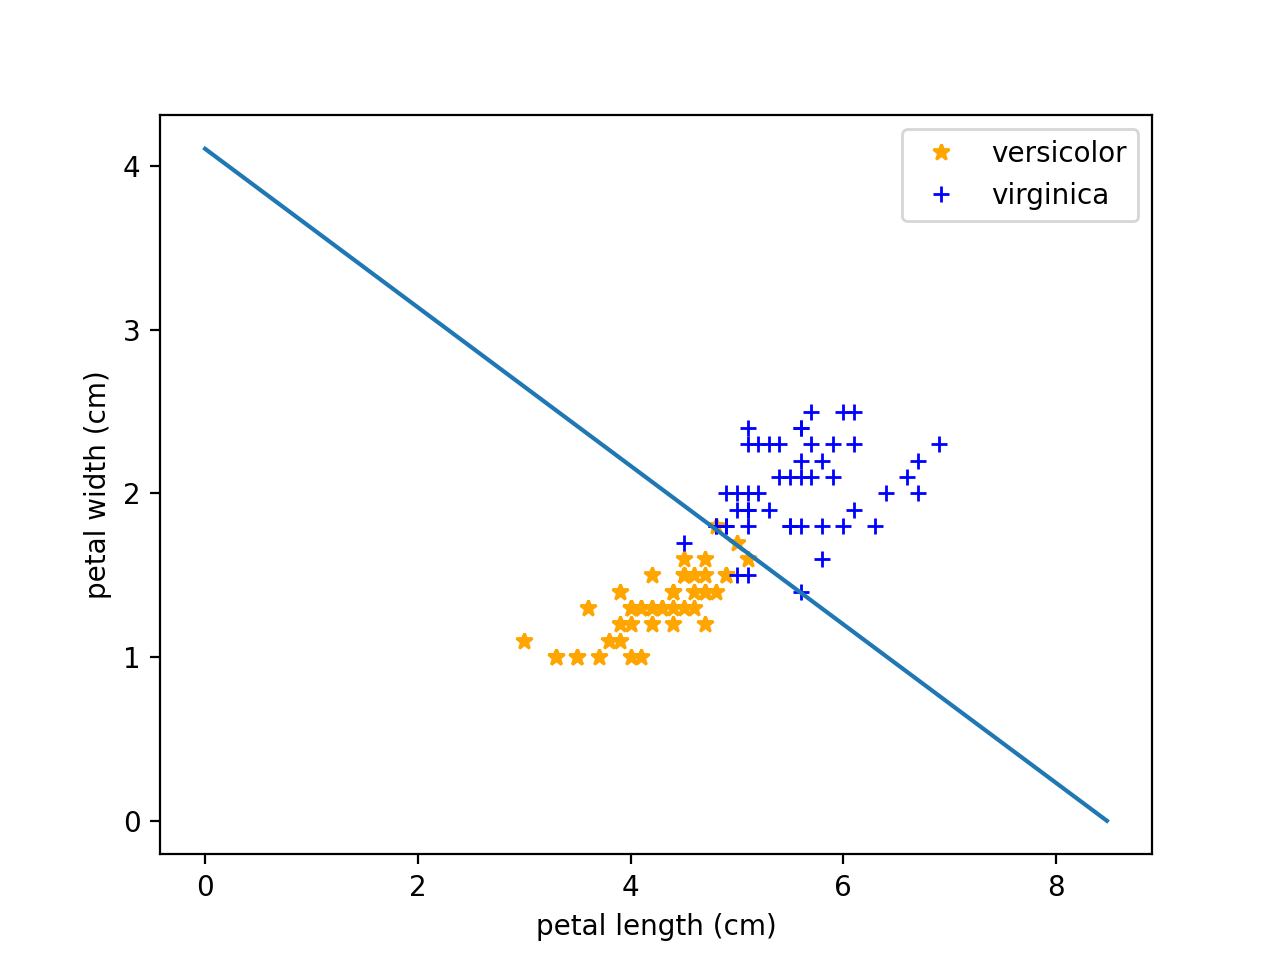
\includegraphics[scale=0.6]{fig/p2_b1.png}
\end{center}

\subsubsection*{2.b.2}
The second set of weights we've chosen is $[-1, 0.7, 2]$. The mean squared error we concluded is 0.48802189762271864. The following figure shows the linear boundary with our chosen set of weights. As we can tell from the graph, the linear boundary does not seperate these two categories 
at all. 
\begin{center}
    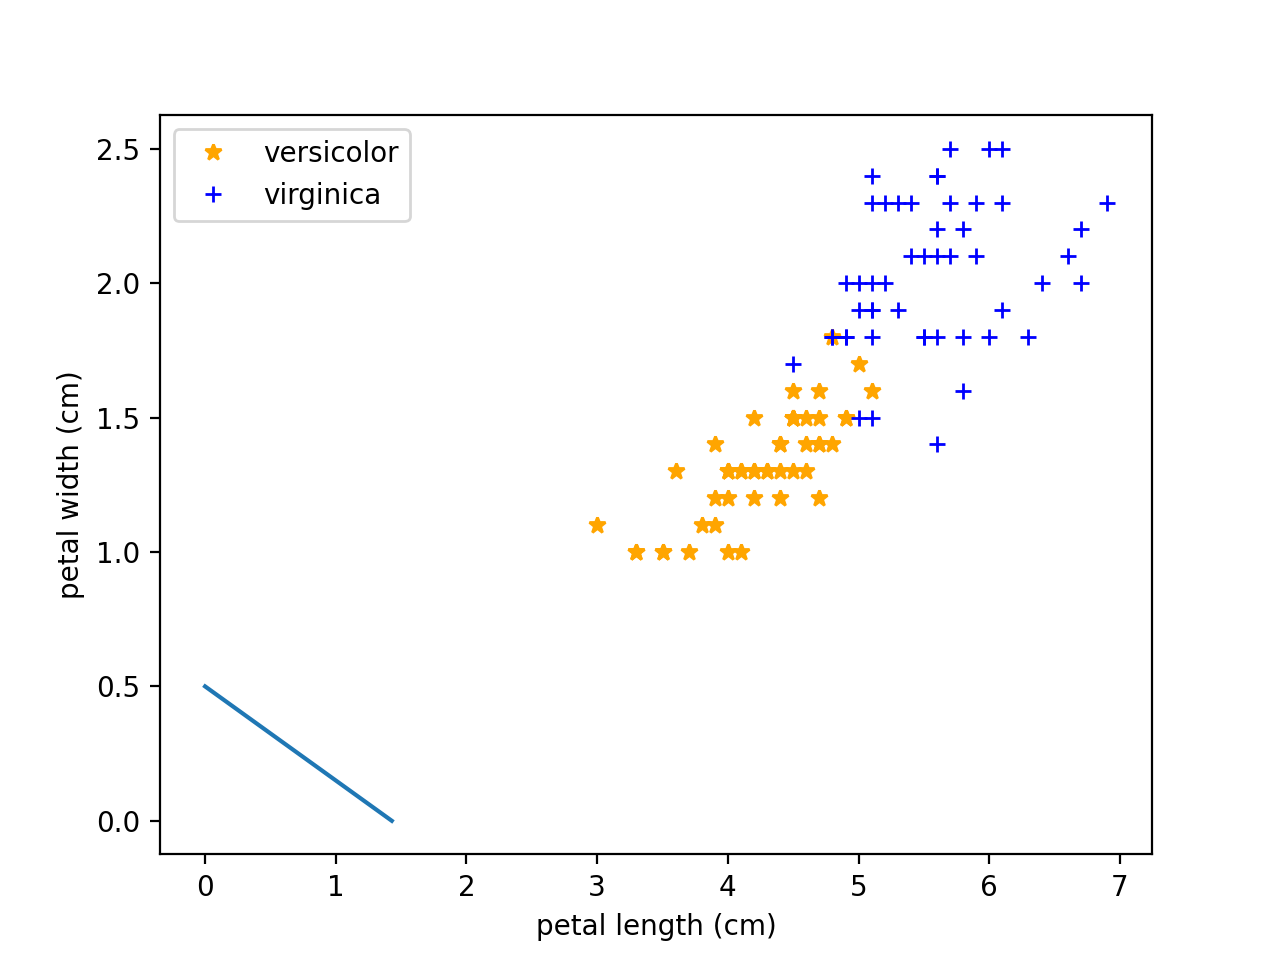
\includegraphics[scale=0.6]{fig/p2_b2.png}
\end{center}

\subsection*{(c)}
To compute the gradient of the objective function, we need to take the derivative of the objective function. Assume \textbf{x$_i$} is the ith row with attribute petal length and petal width such that $x_i = [1,x_{i1},x_{i2}]$($1$ is placed here because $w_0$ requires 1 to be its coefficient). \textbf{w} is the set of weights for the attributes. The logistic function we get is:
\begin{center}
    $\sigma(z) = \frac{1}{1+e^{-z}} = \frac{1}{1+e^{w \cdot x}}$
\end{center}
Therefore, the mean squared function becomes: 
\begin{center}
    $MSE = \frac{1}{N} \sum_{i = 1}^{n}(\sigma(w\cdot x_i)-y_i)^2$
\end{center}
By taking the derivative of this objective function with respect to $w_0$, we have: 
\begin{center}
    $\frac{\partial MSE}{\partial w_0} = \frac{2}{N}\sum_{i=1}^{N}(\sigma(w \cdot x_i)-y_i)\frac{\partial \sigma}{\partial w_0}$ \\ 
    $\frac{\partial MSE}{\partial w_0} = \frac{2}{N}\sum_{i=1}^{N}(\sigma(w \cdot x_i)-y_i)(1-\sigma(w \cdot x_i))(\sigma(w\cdot x_i))\frac{\partial (w\cdot x)}{\partial w_0}$ \\ 
    $\frac{\partial MSE}{\partial w_0} = \frac{2}{N}\sum_{i=1}^{N}(\sigma(w \cdot x_i)-y_i)(1-\sigma(w \cdot x_i))(\sigma(w\cdot x_i))$
\end{center}
Similarly, by only changing the last derivative $\frac{\partial(w\cdot x)}{\partial w_0}$ to $\frac{\partial(w\cdot x)}{\partial w_1}$ and $\frac{\partial(w\cdot x)}{\partial w_2}$, we can compute the derivative of the objective function with respect to $w_1$ and $w_2$:
\begin{center}
    $\frac{\partial MSE}{\partial w_1} = \frac{2}{N}\sum_{i=1}^{N}(\sigma(w \cdot x_i)-y_i)(1-\sigma(w \cdot x_i))(\sigma(w\cdot x_i))x_{i1}$
    $\frac{\partial MSE}{\partial w_2} = \frac{2}{N}\sum_{i=1}^{N}(\sigma(w \cdot x_i)-y_i)(1-\sigma(w \cdot x_i))(\sigma(w\cdot x_i))x_{i2}$
\end{center} 
Therefore, the gradient of MSE is: 
\begin{center}
    $\nabla MSE = \left[\begin{array}{@{}c@{}}
        \frac{\partial MSE}{\partial w_0} \\ \\
        \frac{\partial MSE}{\partial w_1} \\ \\
        \frac{\partial MSE}{\partial w_2} 
        \end{array} \right] = \left[\begin{array}{@{}c@{}}
            \frac{2}{N}\sum_{i=1}^{N}(\sigma(w \cdot x_i)-y_i)(1-\sigma(w \cdot x_i))(\sigma(w\cdot x_i)) \\ \\
            \frac{2}{N}\sum_{i=1}^{N}(\sigma(w \cdot x_i)-y_i)(1-\sigma(w \cdot x_i))(\sigma(w\cdot x_i))x_{i1} \\ \\ 
            \frac{2}{N}\sum_{i=1}^{N}(\sigma(w \cdot x_i)-y_i)(1-\sigma(w \cdot x_i))(\sigma(w\cdot x_i))x_{i2}
        \end{array} \right]$
\end{center}

\subsection*{(d)}
\subsubsection*{scalar form: }
The scalar form of the gradient is computed in Problem 2 (c): 
\begin{center}
    $\nabla MSE = \left[\begin{array}{@{}c@{}}
        \frac{\partial MSE}{\partial w_0} \\ \\
        \frac{\partial MSE}{\partial w_1} \\ \\
        \frac{\partial MSE}{\partial w_2} 
        \end{array} \right] = \left[\begin{array}{@{}c@{}}
            \frac{2}{N}\sum_{i=1}^{N}(\sigma(w \cdot x_i)-y_i)(1-\sigma(w \cdot x_i))(\sigma(w\cdot x_i)) \\ \\
            \frac{2}{N}\sum_{i=1}^{N}(\sigma(w \cdot x_i)-y_i)(1-\sigma(w \cdot x_i))(\sigma(w\cdot x_i))x_{i1} \\ \\ 
            \frac{2}{N}\sum_{i=1}^{N}(\sigma(w \cdot x_i)-y_i)(1-\sigma(w \cdot x_i))(\sigma(w\cdot x_i))x_{i2}
        \end{array} \right]$
\end{center}

\subsubsection*{vector form: }
Let $X = \left[\begin{array}{@{}c@{}}
        x_{11}, x_{12}, 1 \\
        \dots \\
        x_{n1}, x_{n2}, 1
         \end{array} \right]$, which is a matrix represents the attributes(1 corresponds for bias).
Since the term $\frac{2}{N}\sum_{i=1}^{N}(\sigma(w \cdot x_i)-y_i)(1-\sigma(w \cdot x_i))(\sigma(w\cdot x_i))$ is independent of the dimension
$j$ and common for $\frac{\partial MSE}{\partial w_0}$, $\frac{\partial MSE}{\partial w_1}$, and $\frac{\partial MSE}{\partial w_2}$, we can first express 
this term as $z_i = (\sigma(w \cdot x_i)-y_i)(1-\sigma(w \cdot x_i))(\sigma(w\cdot x_i))$. The gradient of MSE becomes: 
\begin{center}
    $\nabla MSE = \frac{2}{m} \left[\begin{array}{@{}c@{}}
                \sum_{i=1}^{N} z_i \\
                \sum_{i=1}^{N} z_{i}x_{i1} \\
                \sum_{i=1}^{N} z_{i}x_{i2}
                \end{array} \right] = \frac{2}{m}\left[\begin{array}{@{}c@{}}
                                     1, \dots, 1 \\
                                     x_{11}, \dots, x_{n1} \\
                                     x_{12}, \dots, x_{n2}
                                     \end{array} \right] \left[\begin{array}{@{}c@{}}
                                                         z_1 \\
                                                         \dots \\
                                                         z_n
                                                         \end{array}\right] = \frac{2}{m}\mathbf{X^{T}}\left[\begin{array}{@{}c@{}}
                                                            z_1 \\
                                                            \dots \\
                                                            z_n
                                                            \end{array}\right] $
\end{center}
Then, we attempt to expand the vector $z_i = \left[\begin{array}{@{}c@{}}
                                             z_1 \\
                                             \dots \\
                                             z_n
                                             \end{array} \right]$ :
\begin{center}
    $z_i = \left[\begin{array}{@{}c@{}}
            (\sigma(\mathbf{w \cdot x_1})-y_1)(1-\sigma(\mathbf{w \cdot x_1}))(\sigma(\mathbf{w\cdot x_1})) \\
            \dots \\
            (\sigma(\mathbf{w \cdot x_n})-y_n)(1-\sigma(\mathbf{w \cdot x_n}))(\sigma(\mathbf{w\cdot x_n})) 
            \end{array} \right]= \left[\begin{array}{@{}c@{}}
                                 \sigma(\mathbf{w \cdot x_1})-y_1 \\ 
                                 \dots \\
                                 \sigma(\mathbf{w \cdot x_n})-y_n
                                 \end{array} \right] \star \left[\begin{array}{@{}c@{}}
                                                           1-\sigma(\mathbf{w \cdot x_1}) \\
                                                           \dots \\
                                                           1-\sigma(\mathbf{w \cdot x_n})
                                                           \end{array} \right] \star \left[\begin{array}{@{}c@{}}
                                                                                     \sigma(\mathbf{w\cdot x_1}) \\
                                                                                     \dots \\
                                                                                     \sigma(\mathbf{w\cdot x_n})
                                                                                     \end{array} \right]$
\end{center}
The $\star$ operation is defined as multiplying the ith row's elements. To simplify the expression, let $\sigma(\mathbf{Xw}) = \left[\begin{array}{@{}c@{}}
                                                                                                         \sigma(\mathbf{w^{T}x_1}) \\
                                                                                                         \dots \\
                                                                                                         \sigma(\mathbf{w^{T}x_n})
                                                                                                         \end{array} \right]$. 
Thus, $z_i$ can be expressed as $z_i = (\sigma(\mathbf{Xw})-\mathbf{y})\star(1 - \sigma(\mathbf{Xw}))\star \sigma(\mathbf{Xw})$. The vector form of gradient can be expressed as: 
\begin{center}
    $\nabla MSE = \frac{2}{m}\mathbf{X^T}(\sigma(\mathbf{Xw})-\mathbf{y})\star (\mathbf{1} - \sigma(\mathbf{Xw}))\star \sigma(\mathbf{Xw})$
\end{center}

\subsection*{(e)}
The code we used to calculate the gradient is as following: 
\begin{lstlisting}[language=Python, caption=Calculate Gradient]
def summed_gradient(x, w0, w1, w2, y): 
    sigmoid_list = []
    n = len(x)
    error_list = []
    coefficient_list = []
    x = x.values.tolist()
    y = y.tolist()
    for i in range(len(x)): 
        sigmoid_list.append(one_layer_network(w0, w1, w2, x[i][0], x[i][1]))
        error_list.append(sigmoid_list[i] - y[i])
        coefficient_list.append(error_list[i] * sigmoid_list[i] * (1 - sigmoid_list[i]))
    # number of rows = number of rows in data vectors, number of columns = number of columns in data vector + 1 since 1 for bias coefficient
    temp_matrix = np.ones((len(x), len(x[0]) + 1))
    temp_matrix[:, 1:] = x
    sum_term = np.zeros((len(x), len(x[0]) + 1))
    for i in range(len(coefficient_list)):
        sum_term[i] = (2/n) * temp_matrix[i] * coefficient_list[i]
    return np.sum(sum_term, axis = 0)
\end{lstlisting}
Let step size = 0.01. With the input weight $[w0, w1, w2] = [-5, 0.5, 2]$, we concluded the following table for the illustration of how the decision boundary changes for a small step: 
\begin{center}
    \begin{tabular}{| c | c | c |}
        \hline
        & old data & adjusted data\\
        \hline
        weights & [-5, 0.5, 2] & [-5.00080742  0.49665344  1.9989812] \\
        \hline
        MSE & 0.48802189762271864 & 0.4879972995169846 \\
        \hline
        decision boundary & m = -0.35, b = 0.5 & m = -0.3497940478, b = 0.500093299\\
        \hline
    \end{tabular}
\end{center}
As we can tell from the table, the mean squared error reduced a little bit as we made a small step. To visualize the change of decision boundary, please refer to the following graph: 
\begin{center}
    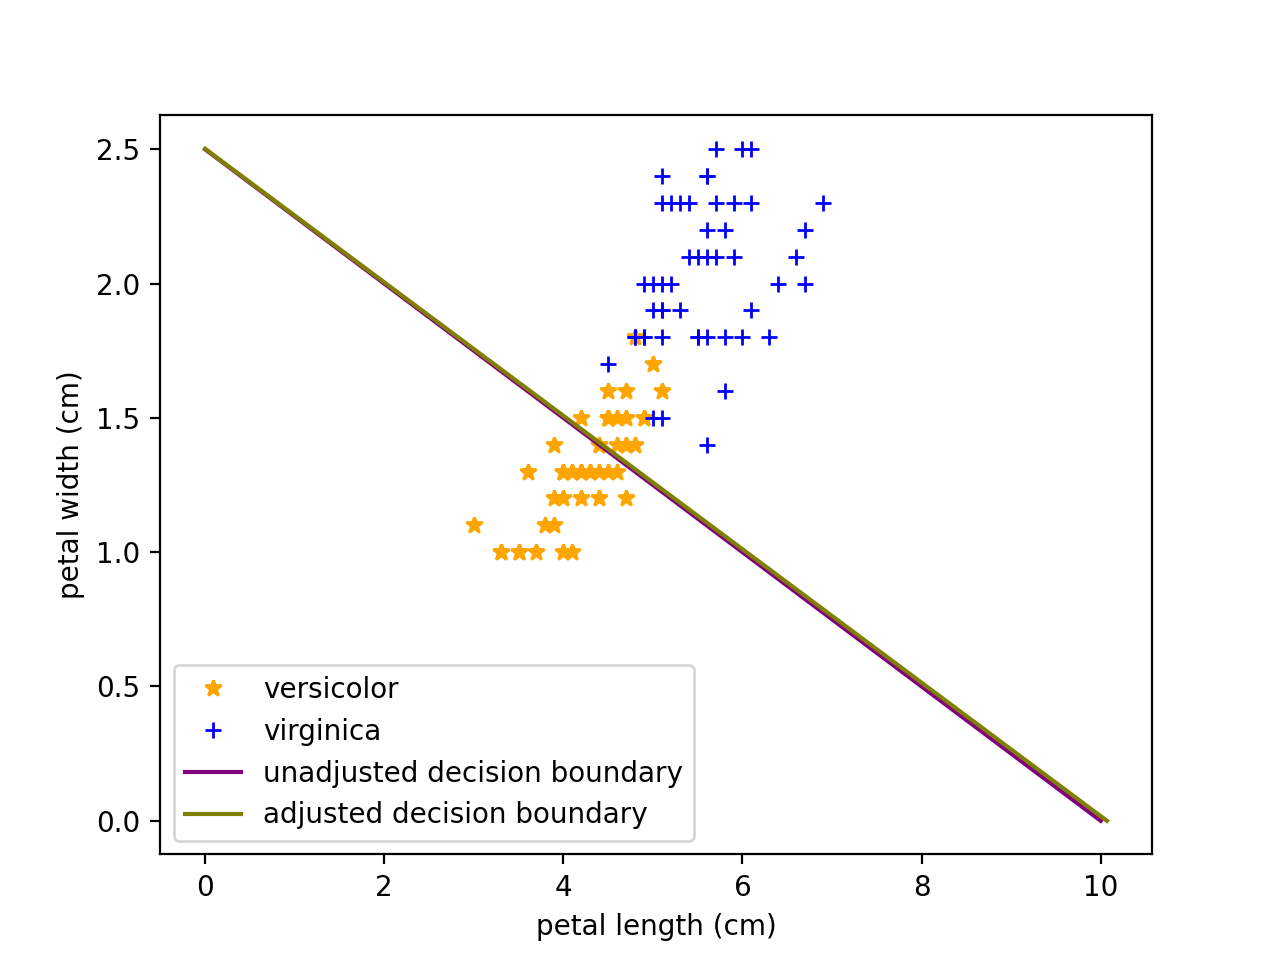
\includegraphics[scale=0.6]{fig/p2e1.png}
\end{center}
Since the small step is kind of hard to tell, we run this process for $10000$ times in order to enlarge the difference. The following two graphs show the decision boundary before the
adjustment and after the adjustment: 
\begin{center}
    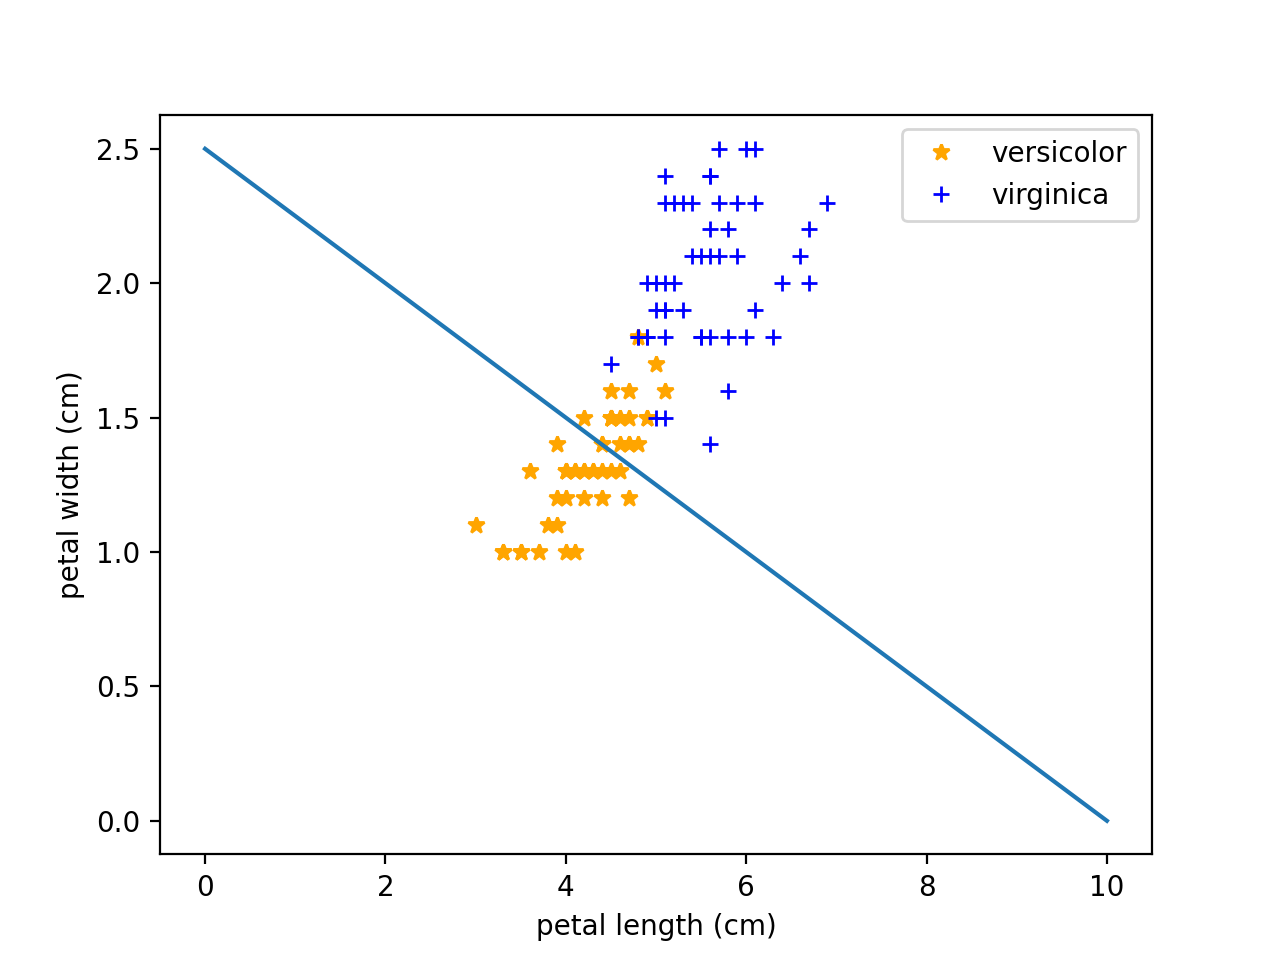
\includegraphics[scale=0.4]{fig/p2e2.png} 
    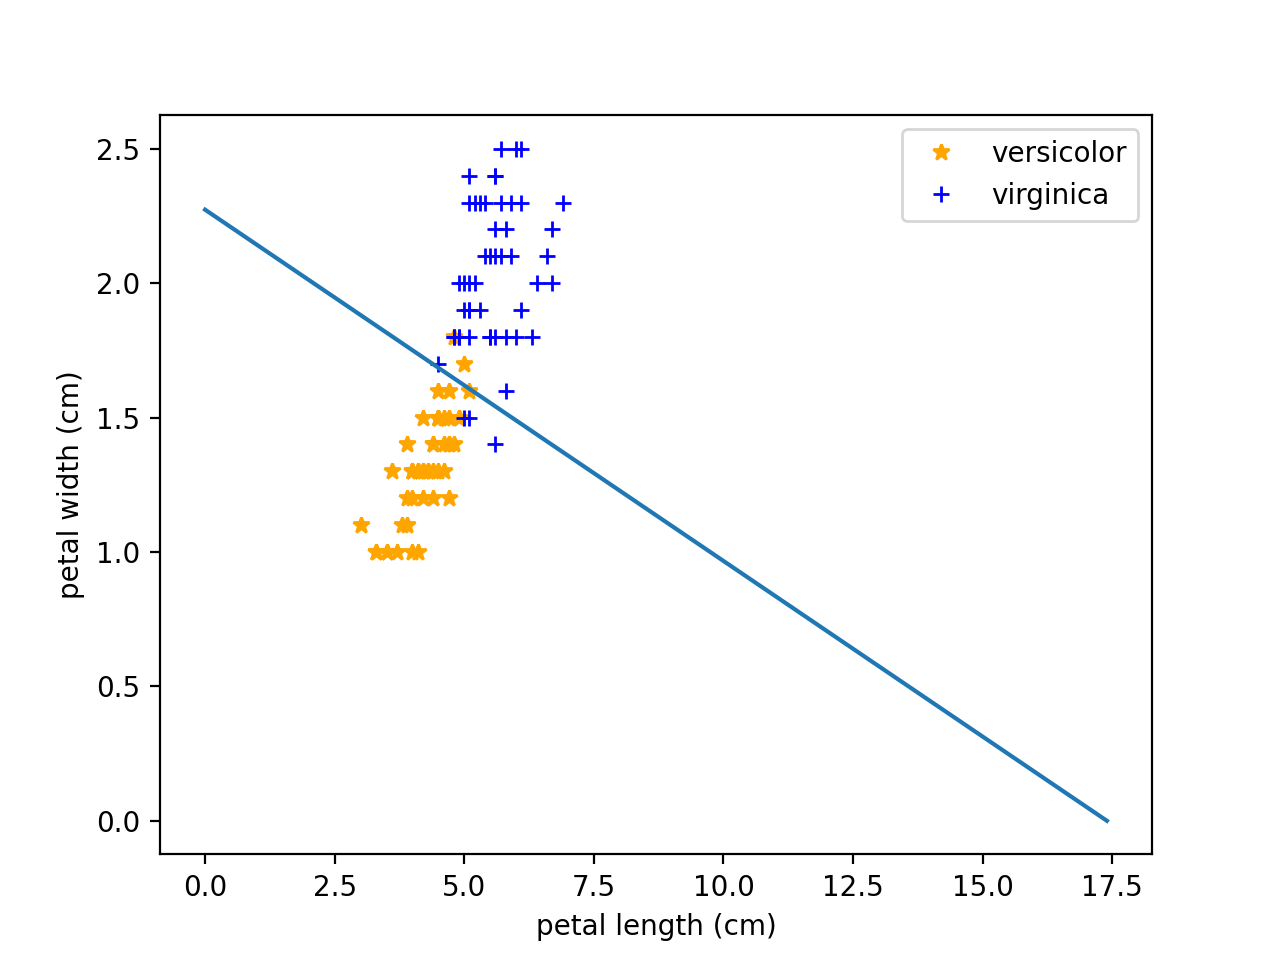
\includegraphics[scale=0.4]{fig/p2e3.png}
\end{center}
The code we used for this illustration is: 
\begin{lstlisting}[language=Python, caption=Illustration of the Change of Gradient]
def illustrate_summed_gradient(x, w0, w1, w2, y):
    num_of_iter = []
    for i in range(10000):
        num_of_iter.append(i+1)
        temp1, temp2, temp3 = summed_gradient(x, w0, w1, w2, y)
        w0 = w0 - 0.01 * temp1
        w1 = w1 - 0.01 * temp2
        w2 = w2 - 0.01 * temp3
    plot([0,-w0/w1],[-w0/w2,0])
\end{lstlisting}

\section*{Problem 3: }
\subsection*{(a)}
The code for gradient descent is as following: 
\begin{lstlisting}[language=Python, caption=Gradient Descent]
def gradient_descent(a, b, x, w0, w1, w2, y): 
    precision = 0.001 # mse we would like to reach
    max_iters = 20000 # max number of iterations
    iteration_counter = 0
    step_size = 0 # using armijo to update
    return_w = []
    current_w = [w0,w1,w2]
    current_mse = mean_square_error(x, w0, w1, w2, y)
    current_sum_g = summed_gradient(x, w0, w1, w2, y)
    improv_checker = 1 # check whether performed better
    # if current mse > the precision we defined and the number of iteration does not exceed the max iteration execute the gradient descent
    while mean_square_error(x, w0, w1, w2, y) > precision and iteration_counter < max_iters:
        if improv_checker > 0:
            return_w = current_w
        iteration_counter += 1
        temp0, temp1, temp2 = summed_gradient(x, w0, w1, w2, y)
        step_size = armijo_updating(a, b, x, y, w0, w1, w2)
        w0 = w0 -  step_size * temp0
        w1 = w1 -  step_size * temp1
        w2 = w2 - step_size * temp2
        current_w = [w0,w1,w2]
        next_mse = mean_square_error(x, w0, w1, w2, y)
        improv_checker = current_mse - next_mse
        current_mse = next_mse
        current_sum_g = summed_gradient(x, w0, w1, w2, y)
        print(w0, w1, w2, mean_square_error(x, w0, w1, w2, y))
        if improv_checker > 0:
            return_w = current_w
    plot([0,-w0/w1],[-w0/w2,0])
    print("MSE: ", mean_square_error(x, w0, w1, w2, y))
    return return_w
\end{lstlisting}
The basic idea is to specify a precision(in this case, mean squared error) and maximum number of iterations we would like to perform. We use the 
summed\_gradient() function and the step size to update the weight in order to reduce the mse. The step size is a dynamic value obtained by using 
Armijo algorithm, which will be illustrated in section 3.d. \\
The following graph is a sample result using the gradient\_descent() function on the example in section 2.b.2.:
\begin{center}
    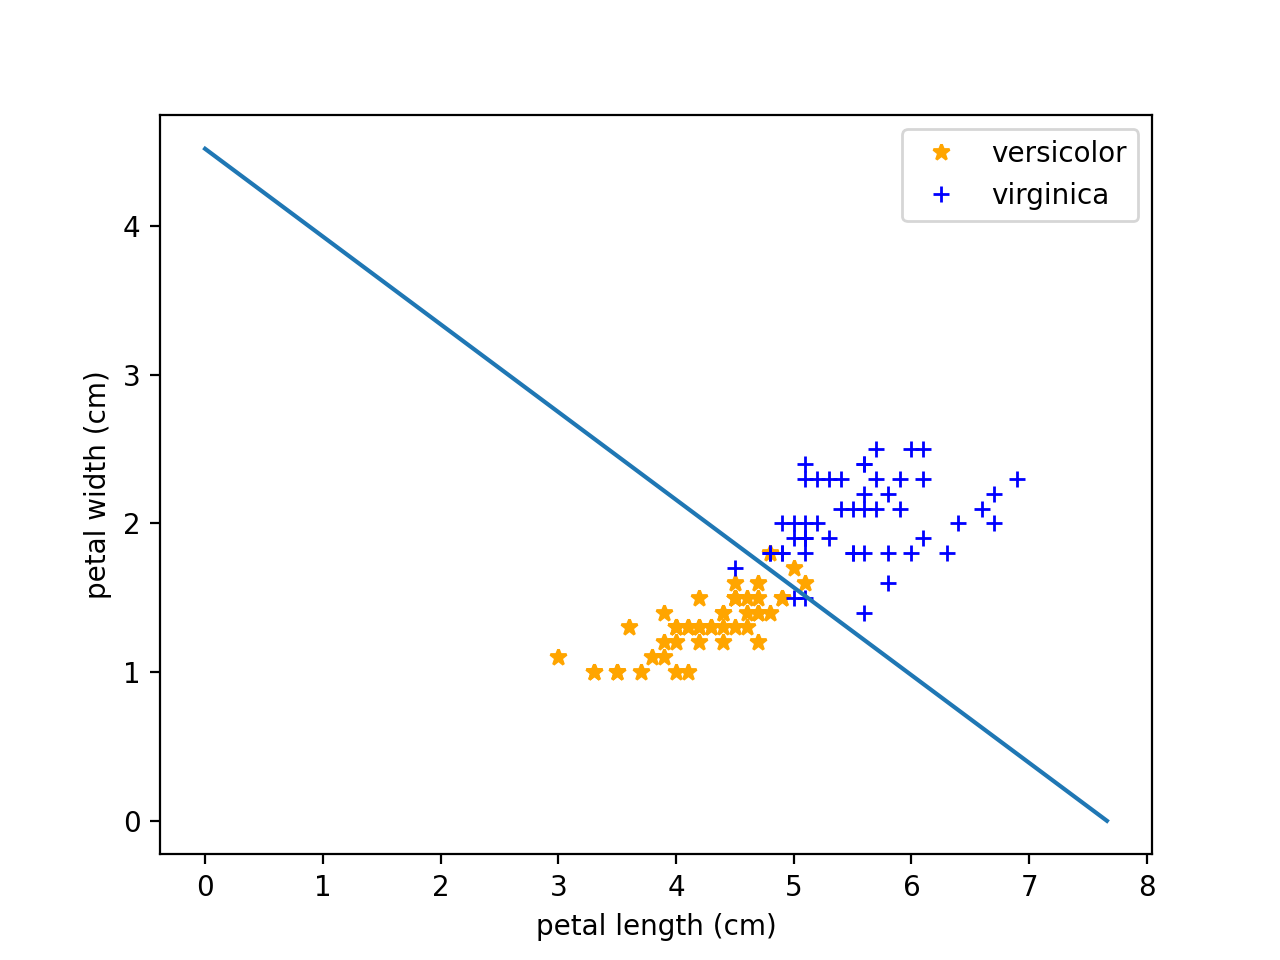
\includegraphics[scale=0.5]{fig/p3a1.png}
\end{center}

\subsection*{(b)}
Since we need to plot the objective function, we revised the code in section 3.a by adding a return element $mse\_list$, which is a list storing the mean 
squared error after each iteration.
\begin{lstlisting}[language=Python, caption=Visualize the Change of Decision Boundary and Objective Function]
def plot_gradient_descent(a, b, x, w0, w1, w2, y):
    df = read_data()
    versicolor = df[df['species']=='versicolor']
    virginica = df[df['species']=='virginica']
    plt.plot(versicolor["petal_length"], versicolor["petal_width"], '*',label="versicolor", color = 'orange')
    plt.plot(virginica["petal_length"], virginica["petal_width"], '+',label="virginica", color = 'blue')
    # plot the decision boundary
    plt.xlabel("petal length (cm)")
    plt.ylabel("petal width (cm)")
    plt.plot([0, -w0/w1],[-w0/w2, 0], label="initial boundary", color='purple')
    mid_w, mse_list = gradient_descent(1, 0.5, 10000, 0.001, x, w0, w1, w2, y)
    mid_w0, mid_w1, mid_w2 = mid_w[0], mid_w[1], mid_w[2]
    plt.plot([0, -mid_w0/mid_w1],[-mid_w0/mid_w2, 0], label="middle boundary", color='skyblue')
    fin_w, mse_list = gradient_descent(1, 0.5, 20000, 0.001, x, w0, w1, w2, y)
    fin_w0, fin_w1, fin_w2 = fin_w[0], fin_w[1], fin_w[2]
    plt.plot([0, -fin_w0/fin_w1],[-fin_w0/fin_w2, 0], label="final boundary", color='olive')
    # plot the change of objective function
    plt.plot(mse_list)
    plt.xlabel("Number of Iterations")
    plt.ylabel("Objective Function(MSE)")    
    plt.legend()
    plt.show()
\end{lstlisting}
The demonstration of the correctness of this code is in section 3.c. 

\subsection*{(c)}
In this illustration, we select the initial weight to be $[-1, 0.7, 2]$, which is the same example we selected in section 2.b.2. We also select the parameter $a = 1$ and 
$b = 0.5$. The middle boundary for the objective function occurs when the number of iterations is $10000$(since the total number of iterations we select is $20000$).
\begin{center}
    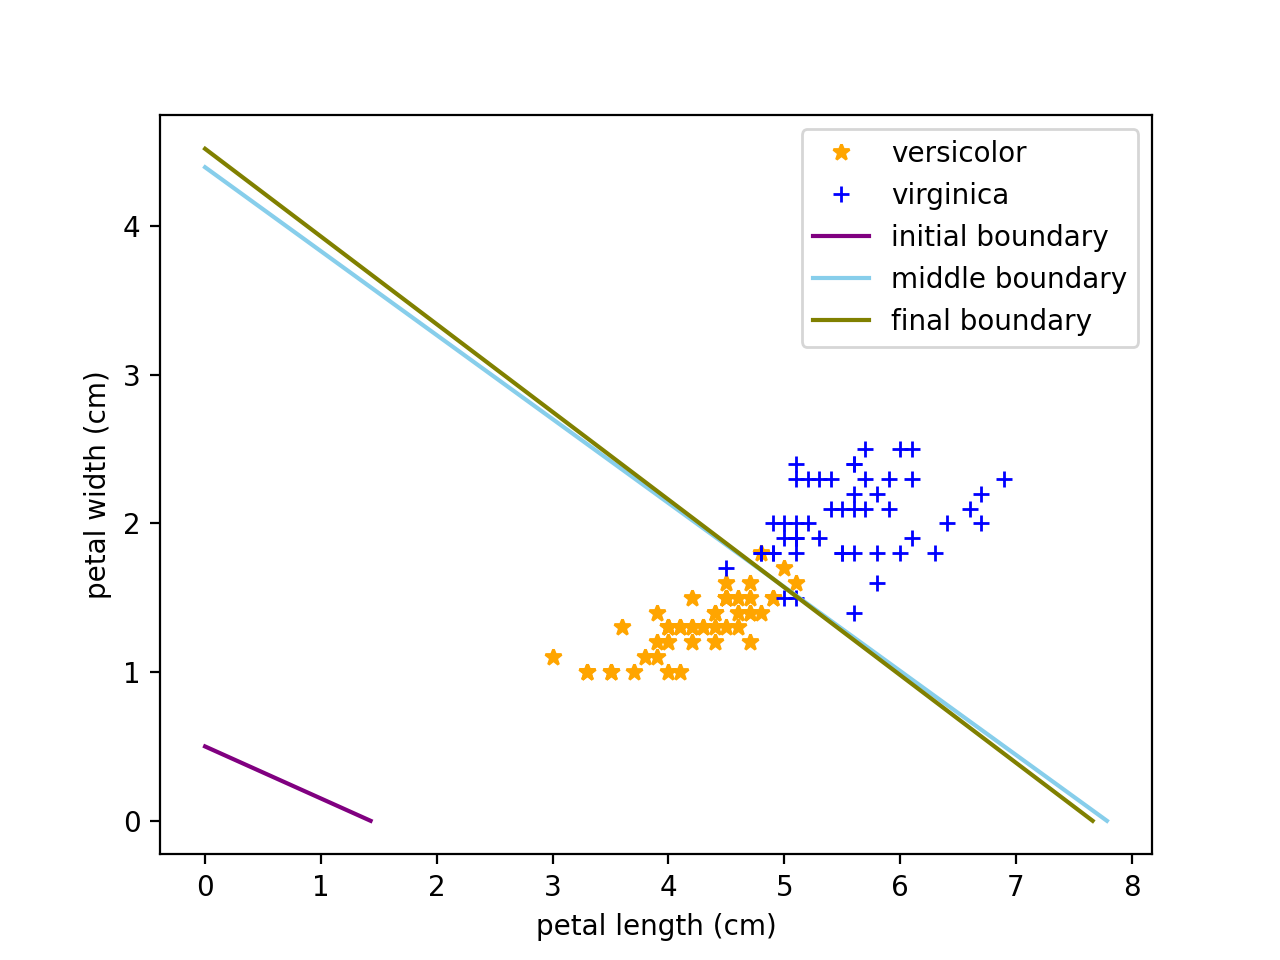
\includegraphics[scale=0.35]{fig/p3b1.png}
    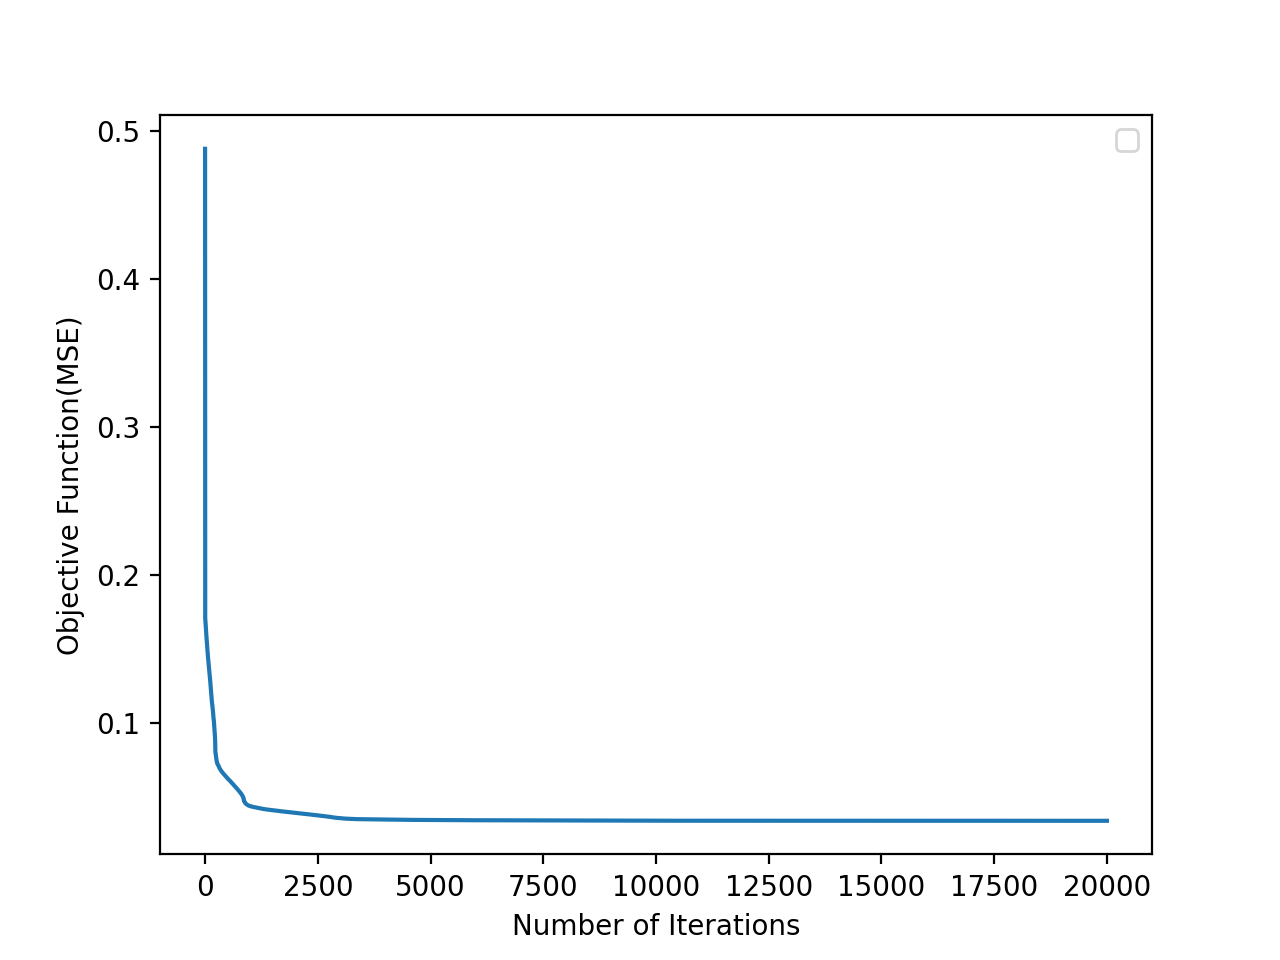
\includegraphics[scale=0.35]{fig/p3b2.png}
\end{center}
To further illustrate the correctness of our code, we select another set of initial weight $[-8, 0.6, 1]$. Select $a = 1$ and $b = 0.5$ and run for $20000$ iterations, we have: 
\begin{center}
    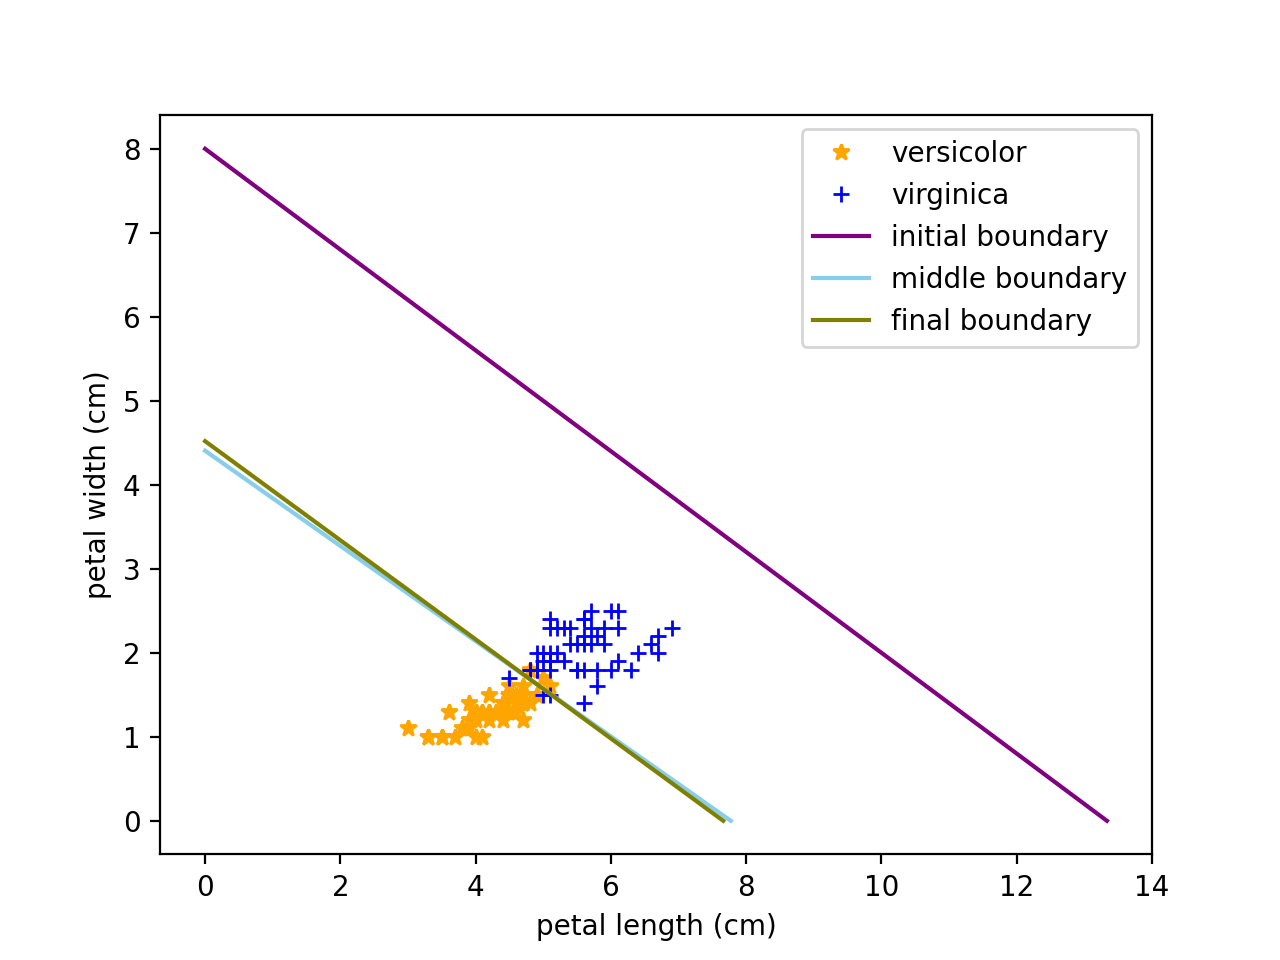
\includegraphics[scale=0.35]{fig/p3c3.png}
    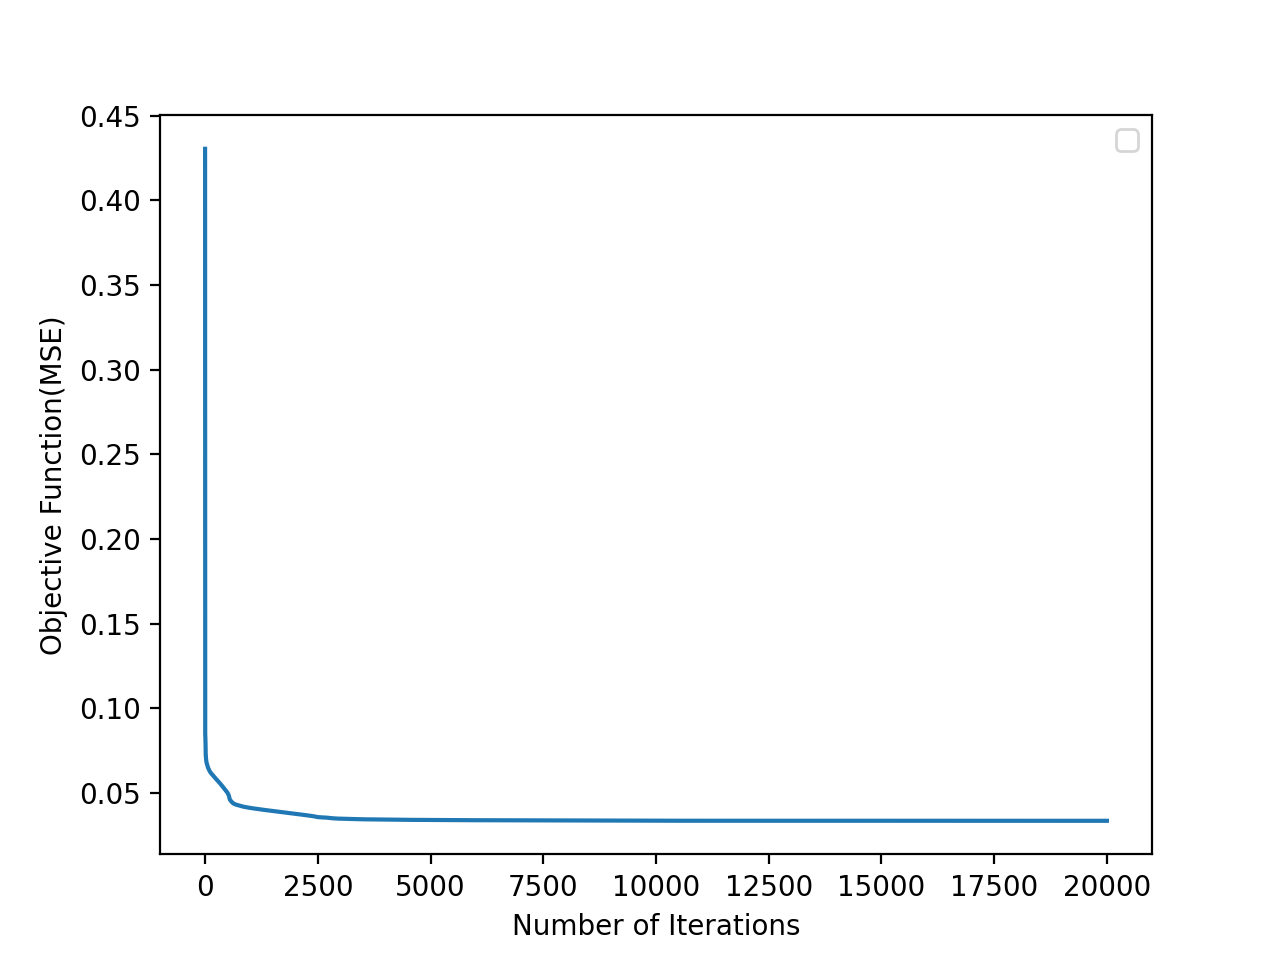
\includegraphics[scale=0.35]{fig/p3c4.png}
\end{center}

\subsection*{(d)}
The choice of gradient step size is important because if the step size is too large, the algorithm will not converge and jump around the minimum;
if the step size is too small, the convergence will take place pretty slowly. Therefore, instead of using a constant step size, we decided to adjusted
our step size while running the algorithm. To choose the step size, we used back-tracking inexact line search with
Armijo rule(please refer to the article: \href{http://www.cmap.polytechnique.fr/~dimo.brockhoff/introoptimization/exercises/09-descentalgorithms-exercise.pdf}{Back-tracking with Armijo rule}). \\
The basic idea is to start with a relatively large step size $\alpha_0$ and subtract $\beta^k\alpha$ for $k = 1$ to $n$ until a stopping condition(in this case, smaller than a predefined mse) is met. 
Choose the largest step size for $\alpha$. The stopping step can be expressed as the following formula: 
\begin{center}
    $f(\mathbf{x} + \alpha \mathbf{d}) \le f(\mathbf{x}) + \beta \alpha \nabla f(\mathbf{x})^{T}\mathbf{d}$
\end{center}
, where $f$ is the objective function, $d$ is the descent direction, $\alpha$ and $\beta$ are the parameters of Armijo algorithm. For the problem of iris dataset, we can rewrite the above function as following
in order to update the step size: 
\begin{center}
    $f(\mathbf{w - \alpha \nabla\mathbf{w}}) \le f(\mathbf{w})-\beta\alpha\nabla f(\mathbf{x})^{T}f(\mathbf{x})$
\end{center}
, where $w$ is the weight. Since $\beta$ is between $0$ and $1$, while the mean squared error converges to the minimum, the step size decreases. \\
The following code implements the Armijo algorithm: 
\begin{lstlisting}[language=Python, caption=Armijo Updating Step Size]
def armijo_updating(a, b, x, y, w0, w1, w2):
    step_size = a
    gradient = summed_gradient(x, w0, w1, w2, y)
    while mean_square_error(x, w0 - (step_size * gradient[0]), w1 - (step_size * gradient[1]), w2 - (step_size * gradient[2]), y) > mean_square_error(x, w0, w1, w2, y) - (0.5 * step_size * la.norm(gradient) ** 2):
        step_size = step_size * b
    return step_size
\end{lstlisting}
The step size does not assure us to find the global minimum since the step size could be too large for the final step(but by using the Armijo Updating algorithm,
it performs much better than just select a constant stepping size). Note in the $gradient\_descent$ function, if the final iteration makes an improvement, then we will adopt it; otherwise, we won't. This ensures us to be as close to the global minimum of the objective function
as possible. 

\subsection*{(e)}
The stopping criterion(in our code, it is represented as precision) we chose is $0.001$ for precision(or tolerance of error) and $20000$ for the number of iterations because it is a good balance between the time consumed to run the code and the precision of the decision boundary. As we illustrated in the graphs above, a precision of 
$0.001$ is sufficient to classify the categories relatively accurate. If we select a much smaller precision or a much larger number of maximum iterations, it will take too much time to make just a little bit of improvement. As we can see from the graph of objective functions, after a certain threshold of 
number of iterations, the improvement we made is actually trivial. 

\section*{Problem 4(Extra Credit): }
The following two graphs visualize the classification of iris dataset with 4 attributes: 
\begin{center}
    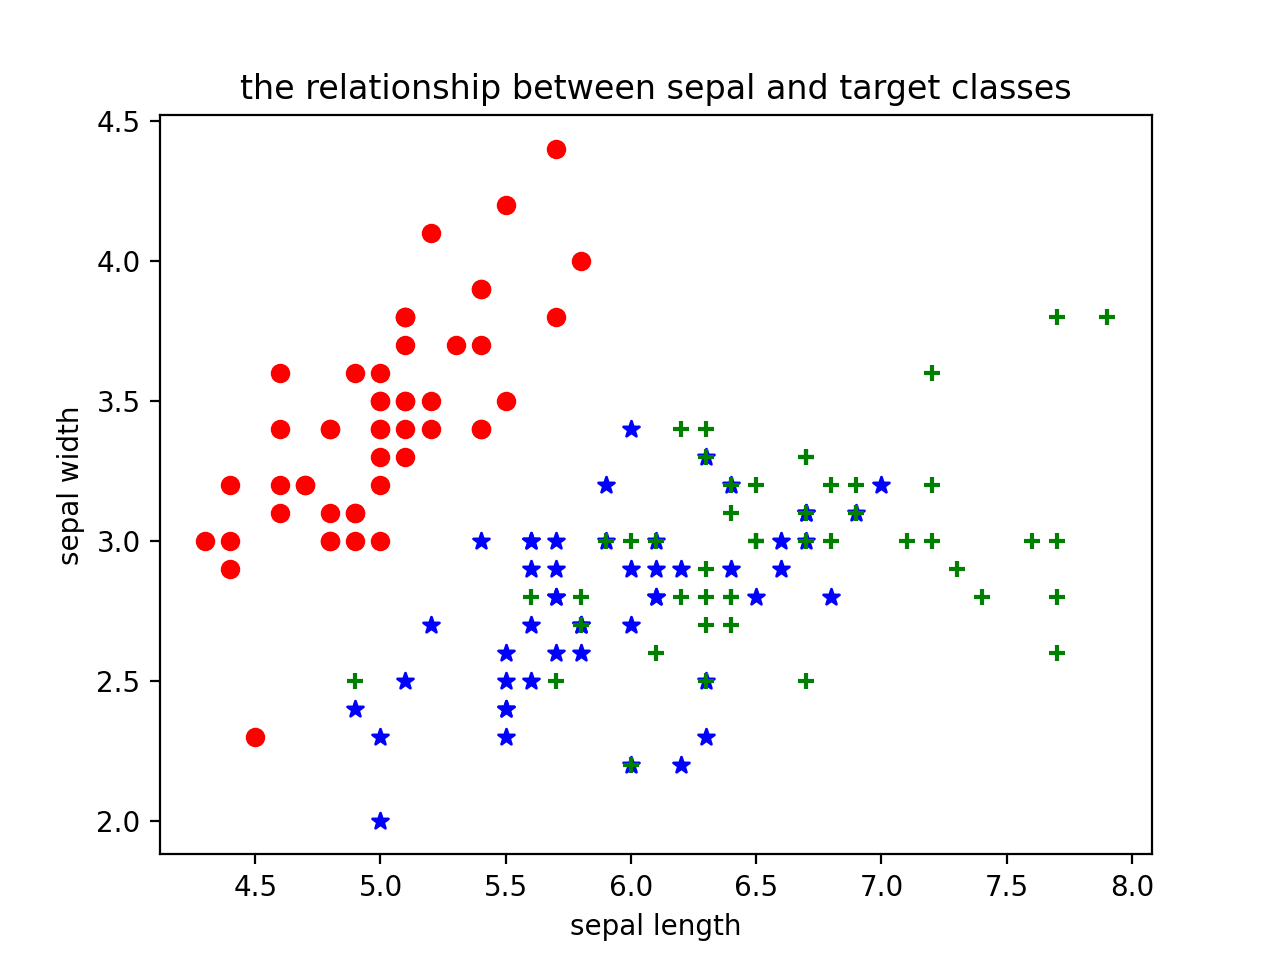
\includegraphics[scale=0.35]{fig/ec1.png}
    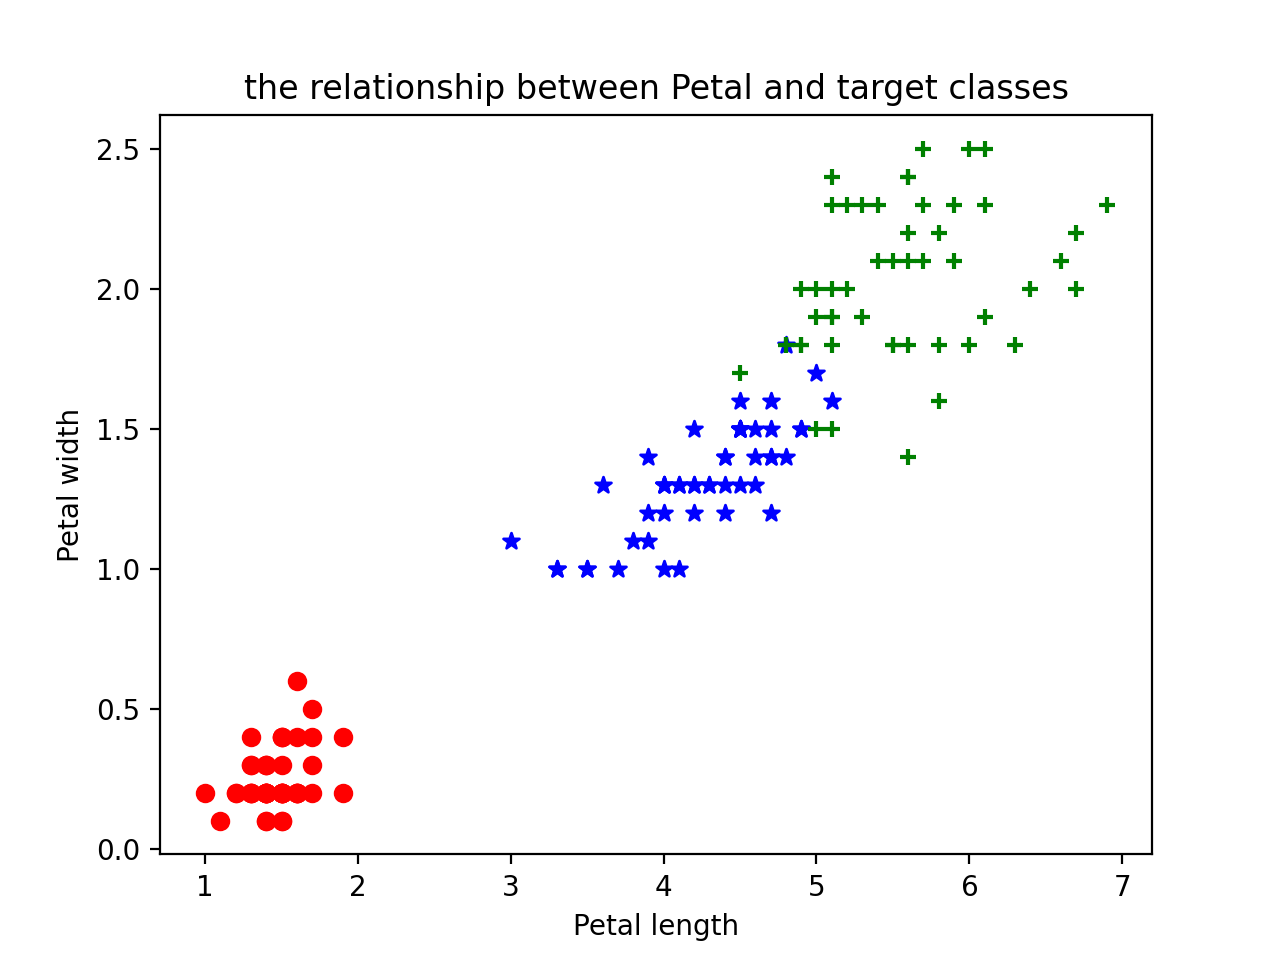
\includegraphics[scale=0.35]{fig/ec2.png}  
\end{center}
To categorize 3 classes by $4$ attributes, we used \textbf{Support Vector Machine(SVM)}, which is a tool to find a hyperplane in a multi-dimensional space that distinctly classifying the data points. 

\subsection*{4.1 Brief Explanation of the Idea Behind SVM}
The general idea is to start with data from a lower dimension and map our space to a higher dimension in order to find a hyperplane to classify the data points. Here is a simple example: the following graph is a number axis with 1-dimension, where the red points and the green points are two different classes we would like to classify and 
the orange line is the decision boundary we compute to seperate the data points. However, in this case, it is hard to find a boundary which precisely seperates these two classes since no matter where we put the decision boundary, the number of misclassifications would be large. 
\begin{center}
    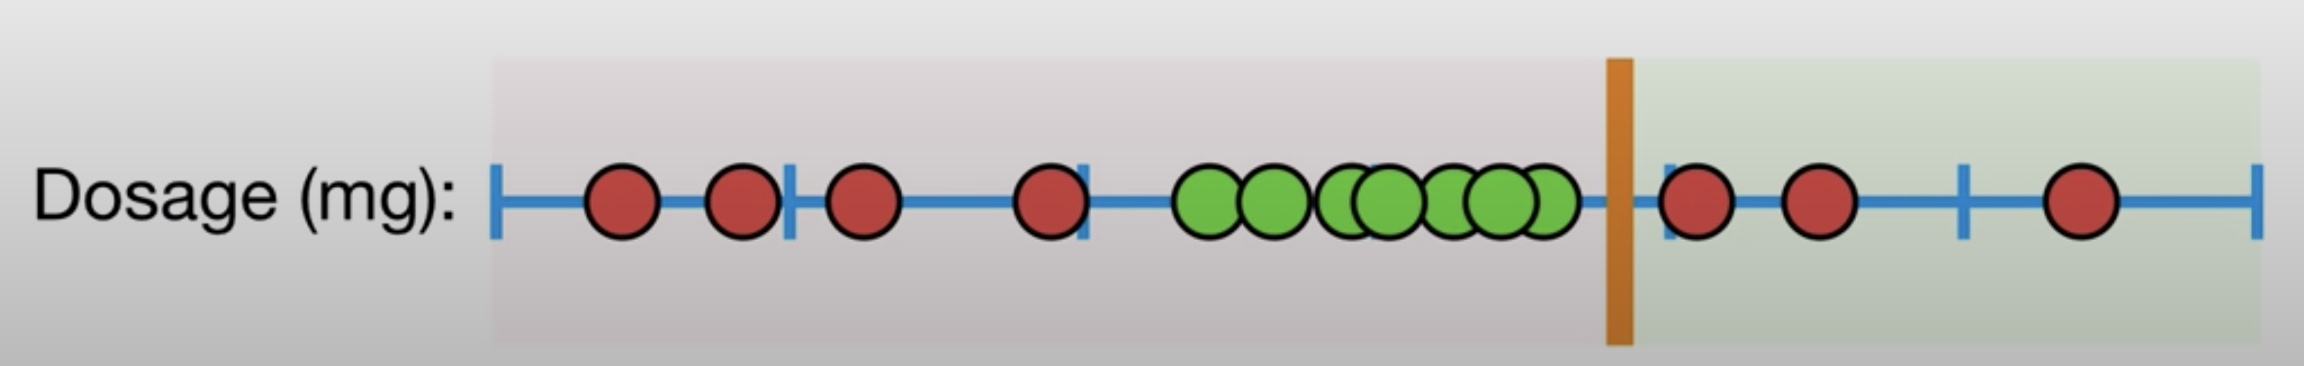
\includegraphics[scale=0.3]{fig/ec_num_axis.png}
\end{center}
In this case, we will add another dimension by squaring the coordinates as $y$, as illustrated in the following graph: 
\begin{center}
    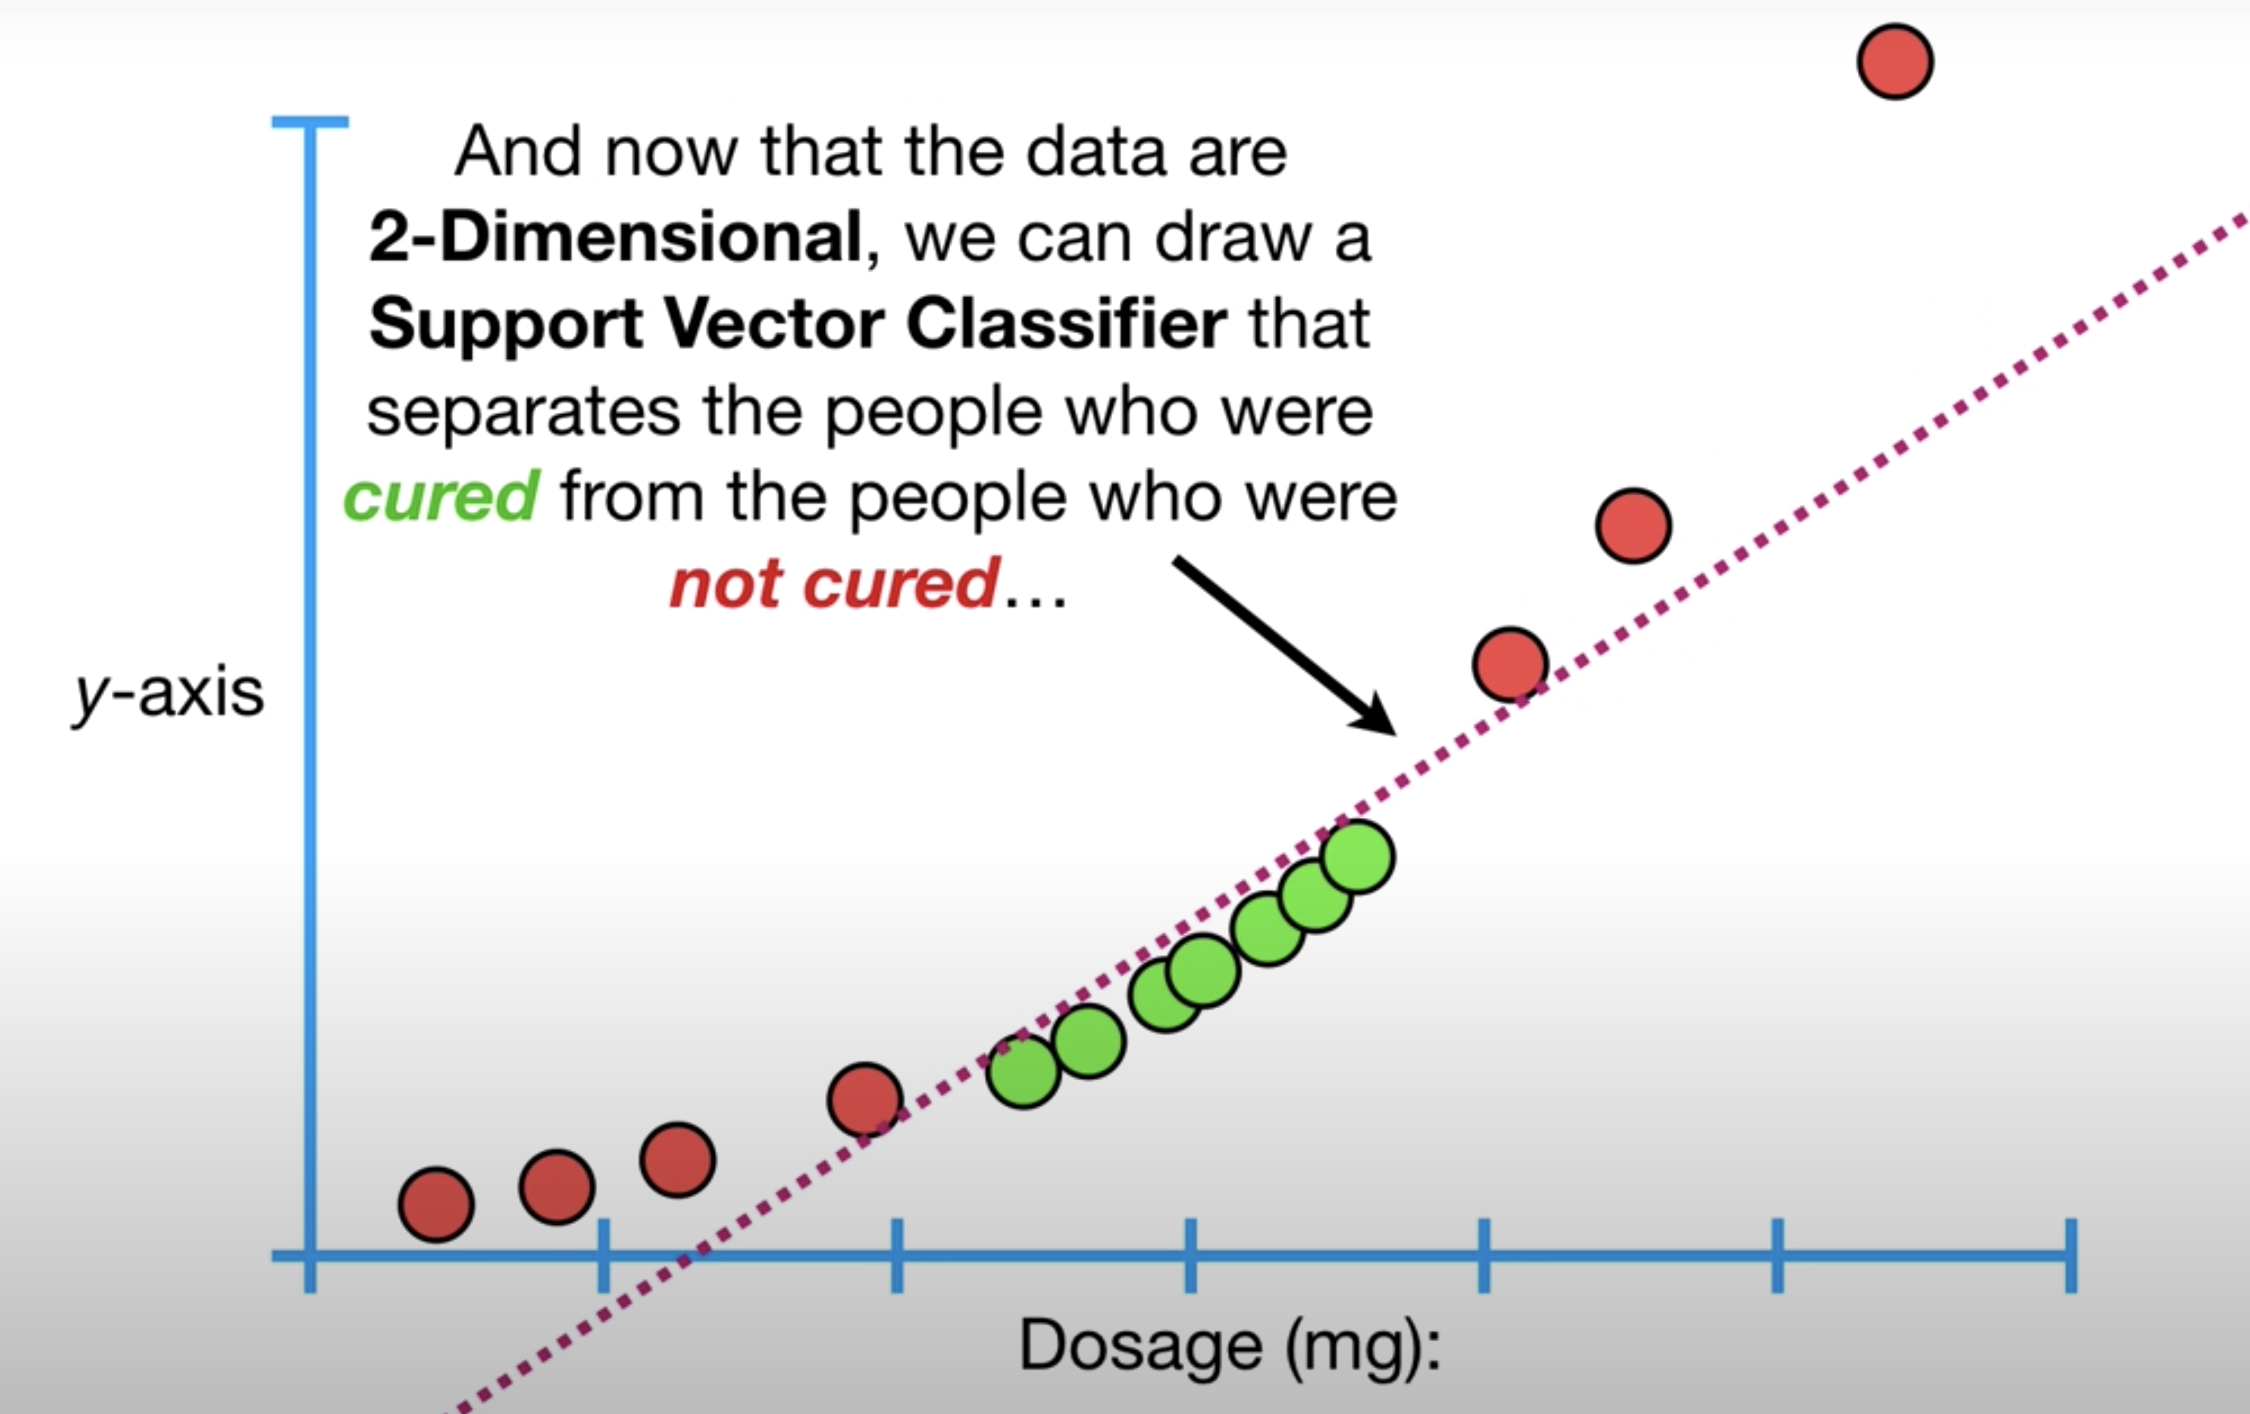
\includegraphics[scale=0.25]{fig/ec_2d.png} \\
\end{center}
The transformation to a higher dimension makes it easier and more accurate for us to find a decision boundary. \\
Note that in the example, we randomly choose a polynomial function to transform the data from 1-dimension to 2-dimension(by squaring their coordinates). There are actually more than one way to transform those data points. In SVM, we use a \textbf{kernel function} to specify how the data will be transformed to a higher dimension. From the link 
\href{https://stats.stackexchange.com/questions/152897/how-to-intuitively-explain-what-a-kernel-is}{Kernel Explain}, we found an excellent formal definition of kernel: suppose we have a mapping $\Phi:R^n \rightarrow R^m$ that brings our vectors in $R^n$ to some feature space $R^m$. Then the dot product of $x$ and $y$ in this space is $\Phi(x)^T \Phi(y)$. 
A kernel is a function k that corresponds to this dot product, i.e. $k(\mathbf{x},\mathbf{y}) = \Phi(\mathbf{x})^T \Phi(\mathbf{y})$. In the mini tutorial, we will briefly explore how the selection of different kernel function will affect the accuracy of classification.

\subsection*{4.2 Code Implementation}
We classify the dataset by sepal features and petal features seperately. We split the data and the target each to two parts and get 4 datasets: the training set for data, the training set for target, the test set for data, and the test set for target. There are 3 species, each species have 50 samples. We select the test size to be 0.3, which means 
we put 35 samples of each species in training set, and 15 of each in test set. \\
\begin{lstlisting}[language=Python, caption=Train Test Split]
X_train, X_test, y_train, y_test = train_test_split(iris.data[:,2:], iris.target, test_size=0.3, random_state=0)  #[:,2:]
\end{lstlisting}
\textbf{kernel=`sigmoid'}: $k(\mathbf{x},\mathbf{y}) = tanh(\gamma \cdot \mathbf{x^T}\mathbf{y}+\mathbf{r})$ 
\begin{lstlisting}[language=Python, caption=Sigmoid]
sig_svc = svm.SVC(kernel='sigmoid').fit(X_train, y_train)
\end{lstlisting}
\textbf{kernel=`rbf'}: $k(\mathbf{x},\mathbf{y}) = e^{-\gamma \cdot \left\|\mathbf{x}-\mathbf{y}\right\|^2}$ 
\begin{lstlisting}[language=Python, caption=RBF]
rbf_svc = svm.SVC(kernel='rbf').fit(X_train, y_train)
\end{lstlisting}
\textbf{kernel=`poly'}: $k(\mathbf{x},\mathbf{y}) = (\gamma \cdot \mathbf{x^T y} + \mathbf{r})$
\begin{lstlisting}[language=Python, caption=Poly]
poly_svc = svm.SVC(kernel='poly', degree=3).fit(X_train, y_train)
\end{lstlisting}
For each kernel, the function predicts the species according to the model and then the function visualizes the classification: 
\begin{lstlisting}[language=Python, caption=Prediction]
Z = clf.predict(np.c_[xx.ravel(), yy.ravel()])
\end{lstlisting}
The following code is used to predict species and calculates the correctness of the classfication: 
\begin{lstlisting}
sig_svc_pre = sig_svc.predict(X_test)
acc_sig_svc = sum(sig_svc_pre==y_test)/len(y_test)
rbf_svc_pre = rbf_svc.predict(X_test)
acc_rbf_svc = sum(rbf_svc_pre==y_test)/len(y_test)
poly_svc_pre = poly_svc.predict(X_test)
acc_poly_svc = sum(poly_svc_pre==y_test)/len(y_test)
\end{lstlisting}

\subsection*{4.3 Visualization of Output}
The following two graphs are the output of putting iris dataset into SVM with kernel function equals to `sigmoid', `rbf', and `poly'. As we can see from the data points and the decision boundaries, RBF and Polynomial classify classes much better than Sigmoid. By running an accuracy test, we found Sigmoid only correctly classifies $24.4\%$ of sepal data and $11.1\%$ of petal data.
RBF and Polynomial correctly classify $80\%$ of the sepal data and $97.8\%$ of the petal data. 

\begin{center}
    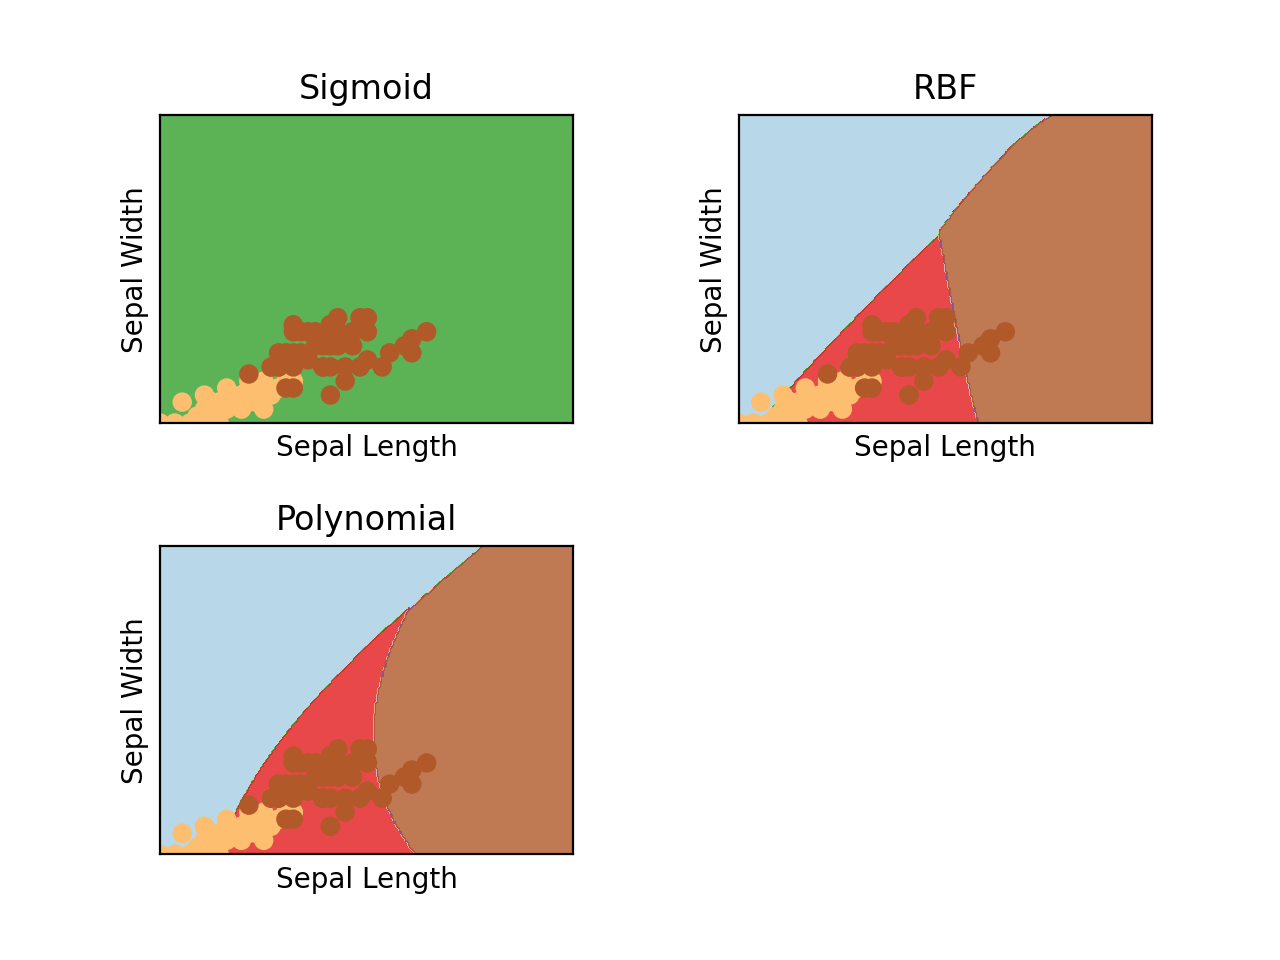
\includegraphics[scale=0.8]{fig/ec3.png}
    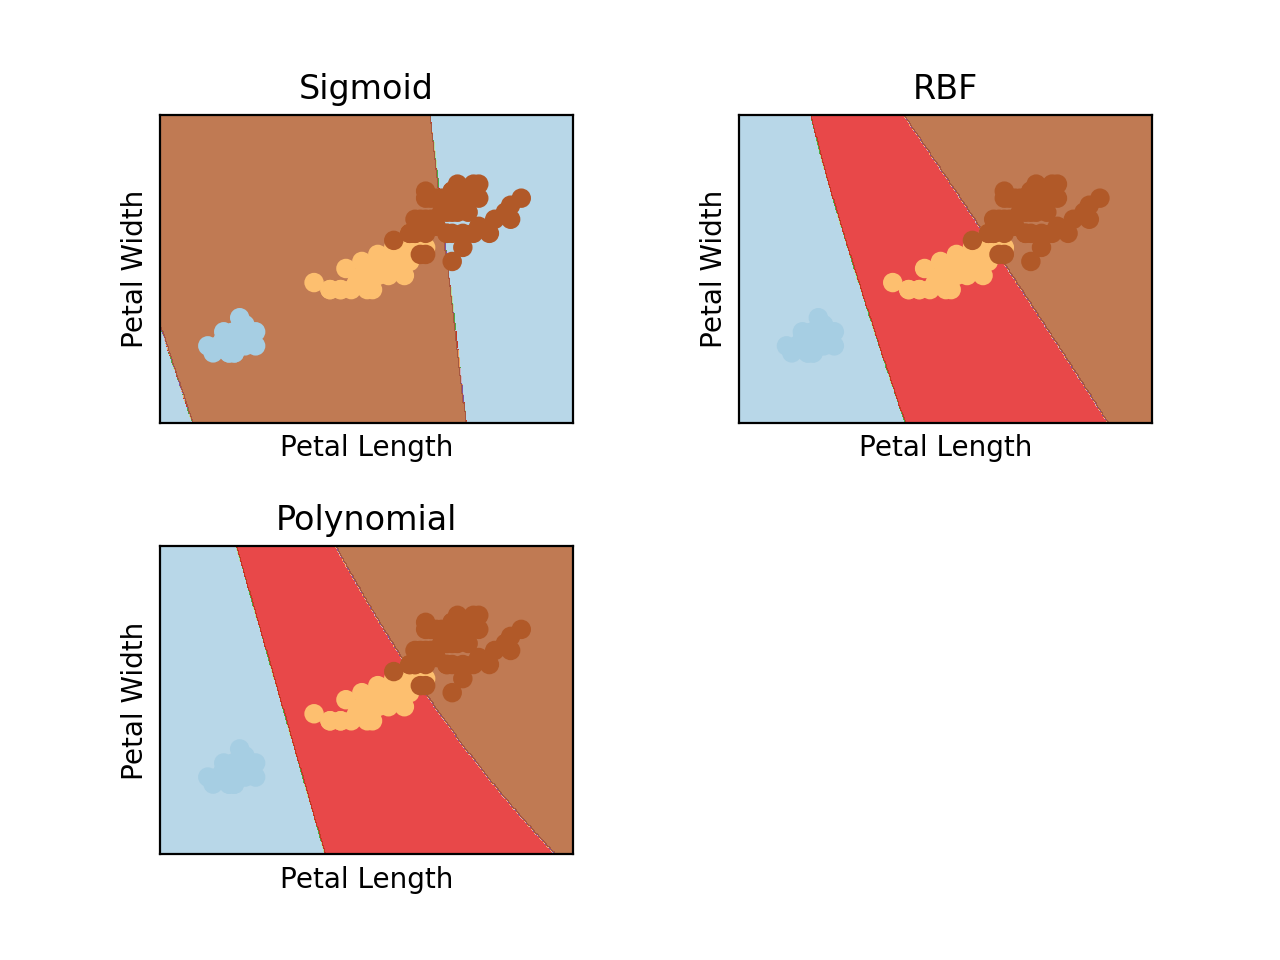
\includegraphics[scale=0.8]{fig/ec4.png} 
\end{center}
The output of test is as below: 
\begin{center}
    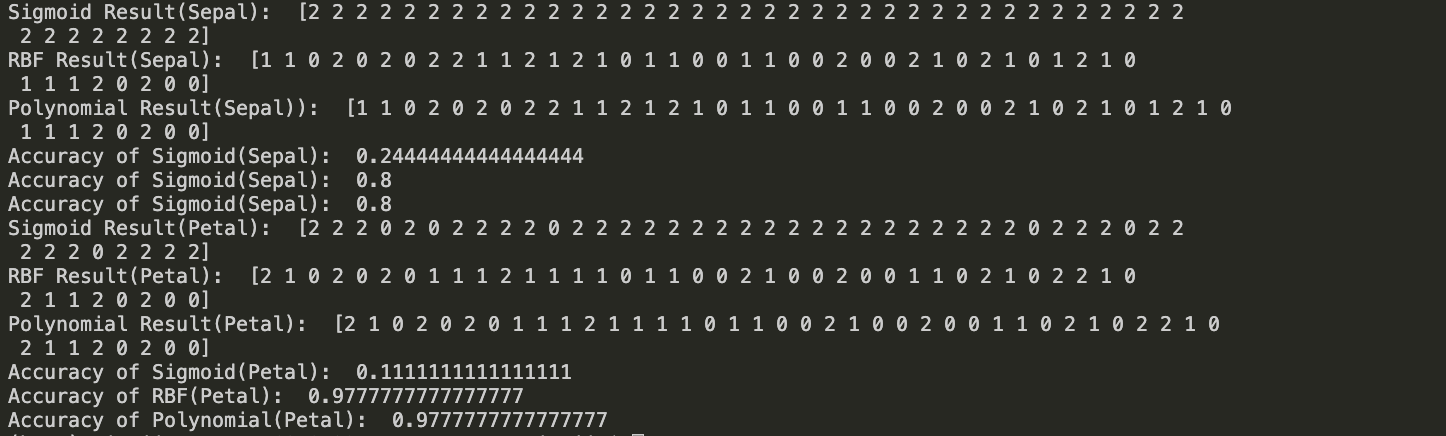
\includegraphics[scale=0.6]{fig/ec_output.png}
\end{center}

\subsection*{4.4 References}
\href{https://www.youtube.com/watch?v=efR1C6CvhmE}{Video to Explain SVM} \\
\href{https://stats.stackexchange.com/questions/152897/how-to-intuitively-explain-what-a-kernel-is}{Kernel Explanation} \\
\href{https://stats.stackexchange.com/questions/90736/the-difference-of-kernels-in-svm}{Different Kernel Function} \\
\href{https://scikit-learn.org/stable/auto_examples/svm/plot_iris_svc.html}{SVM Classification Example}

\end{document}